\graphicspath{{Chapter1/Figs/}}

\section{Introduction}

\begin{frame}\frametitle{DSO Recent Activity}\framesubtitle{}\label{}
\vskip-1.5cm
  Dionysos Satellite Observatory (DSO) of the National Technical University of 
  Athens (NTUA), has developed and maintains an automated processing
  scheme to accommodate the routine analysis of all available continuous GNSS 
  stations in Greece.
  \\
  This daily analysis process is implemented for over five years now (not 
  always continuous though dues to various problems), yielding 
  results which help us further understand the complicated tectonic setting of 
  Greece and nearby regions.
  \\
  Important results, include:
  \begin{itemize}
    \item the recent volcanic activity in \emph{Santorini} (e.g. \cite{papoutsis}),
    \item the 2014 \emph{Kefallonia} earthquakes (e.g. \cite{anastasioukef})
  \end{itemize}
\end{frame}
%
\begin{frame}\frametitle{Motivation}\framesubtitle{}
\vskip-1cm
  % Via our contribution to EUREF and interaction with its community, we hope to:
  Routine GNSS processing and site/network monitoring is crucial, because:
  \begin{itemize}
    \item Greece lies in a region of utmost tectonic and volcanic unrest (e.g. 
      active volcano in Santorini isl.),
    \item results \& products are important to a series of fields spanning 
      the whole range of Geosciences,
    \item helps us follow and apply state-of-the-art technologies in GNSS analysis 
      \& Satellite Geodesy and expand \& modernize our research activity,
    \item contribute to the GNSS/EUREF community and be involved in ongoing/future projects,
    \item improve our academic services (NTUA is a University)
  \end{itemize}
  Throughout the last years, routine processing \& monitoring has hepled us gain 
  a more thorough view of the complex tectonic and volcanic setting of Greece.
\end{frame}

\section{GPS/GNSS Networks in Greece}

\begin{frame}\frametitle{The DataSet}\framesubtitle{}
\vskip-1.5cm
  %To contribute to the Densification we have to establish a credible dataset
  %(network). This has proven to be rather challenging !\\
  Routine processing for precise positioning, assumes a well established, 
  credible dataset (metadata). This has proven to be rather challenging! Lately, 
  the introduction of \texttt{M3G} has provided assistance.\\
  \bigskip
  Currently we process whatever we can get our hands on \ldots\\
  Problems:
  \begin{itemize}
    \item Inhomogenous dataset (\texttt{RINEX} of various versions, raw files, etc).
    \item Various maintainers, different mentalities.
    \item Different aquisition methods/rates.
    \item No log files for mainteners with no geodetic interest (e.g. surveying companies).
    \item Wide variety of equipment (not always included in \texttt{atx} files).
  \end{itemize}
\end{frame}
\note


\begin{frame}\frametitle{Network GREECE}\framesubtitle{}
\vskip-1.5cm

%Network installed/maintained by \texttt{COMET}\footnote{Center for Observation and Modeling of Earthquakes, \url{http://comet.nerc.ac.uk/}} \& \texttt{NTUA}.
\begin{columns}[T] % align columns
\begin{column}{.40\textwidth}
  Network \texttt{Greece} includes the majority of the available sites ($\approx$100)
  but not all of them are (always/currently) active. Various providers but all 
  with geodetic interest \& ecquipment.

  {\small
  \begin{itemize}
    \setlength\itemsep{.1em}
    \item<pro@1-> covers all of Greece
    \item<pro@1-> different (geodetic type) equipment
    \item<pro@1-> credible time-span (early 2004 - now)
    \item<pro@1-> all free available GNSS data
    \item<con@1-> large data gaps \& inactive stations
%    \item<con@1-> needs repairing
\end{itemize}
}
\end{column}%
\hfill%
\begin{column}{.60\textwidth}
 \begin{figure}
 \begin{center}
 \vskip -.2cm
 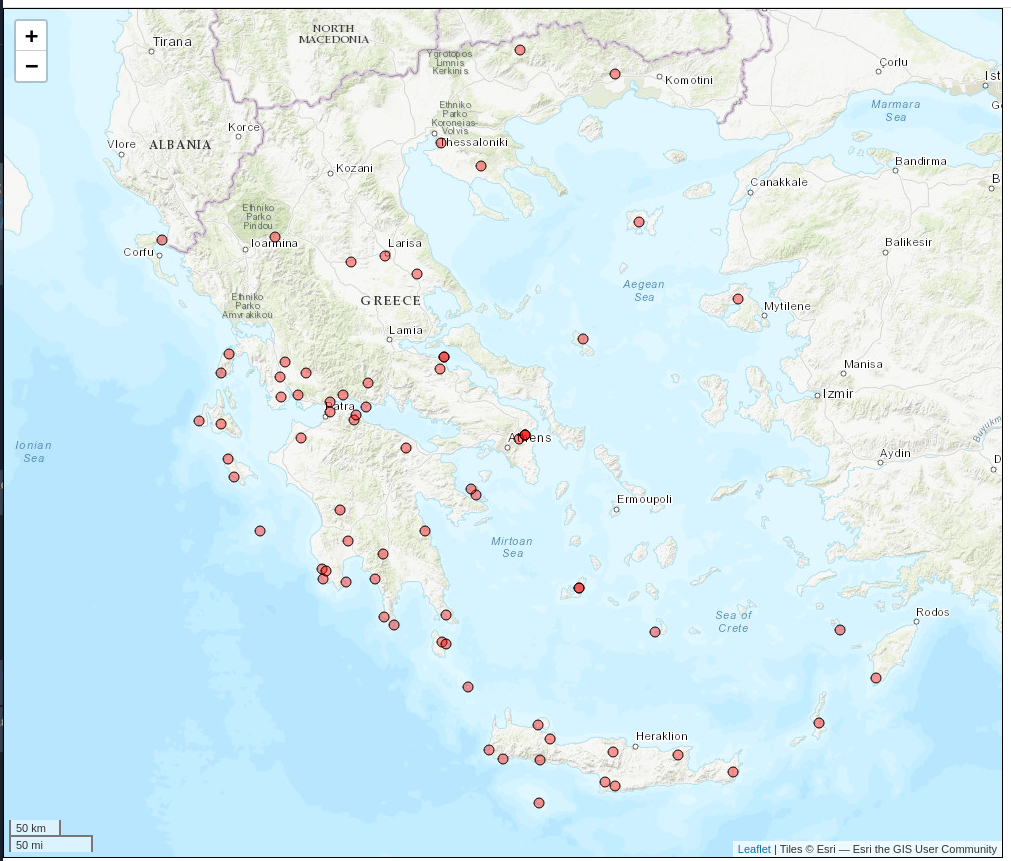
\includegraphics[width=.95\textwidth]{refag_greece_noref.png} %1 2.2 0 0
 \vskip .7cm
% \caption{COMET/NTUA network.}
\href{http://83.212.76.4/abmaps/netmap_noref.php?network=greece}{Network GREECE}
 \label{fig:cometntua}
 \end{center}
 \end{figure}
\end{column}%
\end{columns}
%  \begin{block}{}
%    Can be used for EUREF densification ``as is''.
%  \end{block}
\end{frame}


\begin{frame}\frametitle{Local Networks}\framesubtitle{}
\vskip-.7cm
  %Network installed/maintained by \texttt{CRLab}\footnote{Rift Laboratory \url{http://webobs.crlab.eu/}}. 
  The \texttt{Corinth Rift} network is centered around the Cortinth Gulf, a 
  region of special tectonic interest. Larger site density compared to the 
  rest of Greece.
  \begin{itemize}
    \item<pro@1-> credible time-span
    \item<pro@1-> only covers the Corinth Rift
    \item<con@1-> different providers (including surveying \& cadastral services)
    \item<con@1-> no log files \& equipment changes
  \end{itemize}

 \begin{figure}
 \begin{center}
 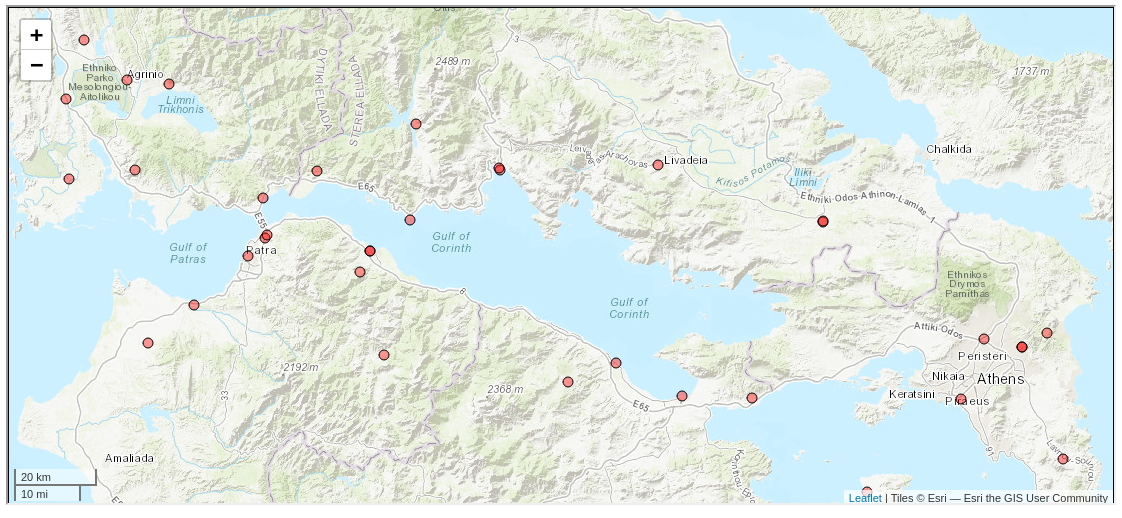
\includegraphics[trim={0cm 2.5cm 0cm 0cm},clip,width=.75\textwidth]{refag_crnet.png}
%  \vskip .6cm
% \caption{EnCeladus network. \url{http://dionysos.survey.ntua.gr/dso/enceladus/}}
  \url{http://dionysos.survey.ntua.gr/dso/enceladus/}
 \label{fig:crlab}
 \end{center}
 \end{figure}
%
%
%  \FourQuad
%  {
%  \textbf{Corinth Rift.}
%  \begin{itemize}
%    \item<pro@1-> credible time-span
%    \item<pro@1-> only covers the Corinth Rift
%    \item<con@1-> inconsistent providers
%    \item<con@1-> no log files \& equipment changes
%  \end{itemize}
%  }
%  {
%
%  }
%  {
%  \textbf{Santorini Network.}
%  Most of the stations installed post-2011 to monitor the \textit{inflation episode}.
%  \begin{itemize}
%    \item<con@1-> localized
%    \item<con@1-> limited time-span
%  \end{itemize}
%  }
%  {
% \begin{figure}
% \begin{center}
% 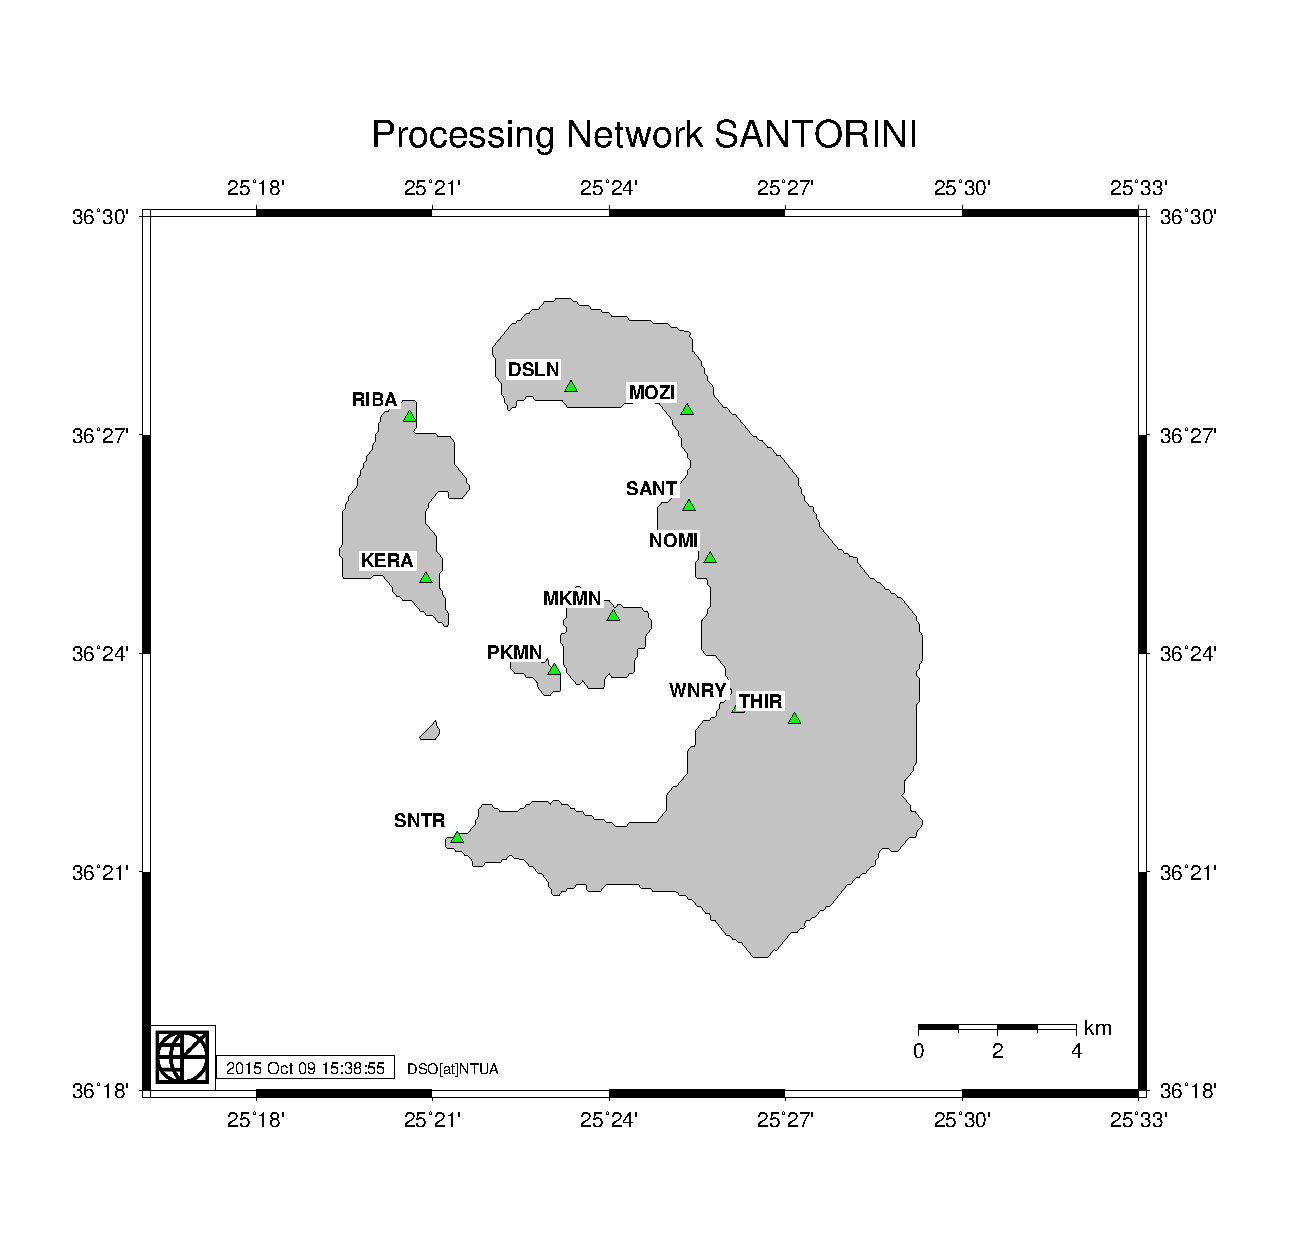
\includegraphics[trim={0cm 2.5cm 0cm 0cm},clip,width=.85\textwidth]{sntrnet.eps}
%  \vskip -.6cm
% \caption{Santorini network.}
% \label{fig:sntrnet}
% \end{center}
% \end{figure}
%  }


\end{frame}


\section{Processing}

\begin{frame}\frametitle{The Scheme}\framesubtitle{}
\begin{columns}[T] % align columns
\begin{column}{.35\textwidth}
\vskip-.5cm
   \footnotesize{The core tool/software is \texttt{Bernese GNSS Software v5.2}\citep{bernese}.\\
   %\medskip
   Integration with
   \begin{itemize}
    \setlength\itemsep{.5em}
     \item \textbf{MySQL} database,
     \item \textbf{Python} module (product/data downloading, pre-processing, 
      driving cron jobs, etc)
     \item \textbf{Time-series} analysis (integrated in routine processing on regular intervals)
     \item \textbf{Strain Rates} via StrainTool (on user demand)
   \end{itemize}}
\end{column}%
\hfill%

\begin{column}{.65\textwidth}
\vskip -.4cm
\begin{figure}
\centering
   \begin{tikzpicture}[ every annotation/.style = {draw,
                      fill = white, font = \large}]

   \path[mindmap,concept color=black!70,text=white,
     every node/.style={concept,circular drop shadow, scale=.4},
     root/.style = {concept color=black!30!red!30,
font=\normalsize\bfseries,text width=5em},
     level 1 concept/.append style={
       font=\normalsize\bfseries, sibling angle=70,text width=7.7em,
       level distance=20mm,inner sep=0pt},
     level 2 concept/.append style={font=\bfseries,level distance=15mm},
   ]

   node[root] {Bernese GNSS Software v5.2} [clockwise from=0]
     child[concept color=red!30] {
       node {pyBern Module} [clockwise from=140]
       child  [color=black!80] { node {github repo} }
       child  { node {handle PCF, BPE, flow-control} }
       child  { node {parsers\\formaters} }
       child  { node {pre-processing \& editing} }
       child  [level distance=13mm] { node {data/product downloading} }
     }
     child[concept color=blue!40] {
       node[concept] {MySQL Database} [clockwise from=-10]
       child { node[concept] {from/to .STA} }
       child { node[concept] {stations/ networks/ products} }
       child [level distance=17mm] { node[concept] {IGS log files} }
     }
     child[concept color=red!60] {
       node[concept] {Cron Jobs} [clockwise from=-40]
       child [level distance=13mm] { node[concept] {final ultra-rapid} }
       child { node[concept] {update ATX, PCV } }
       child { node[concept] {sync with AIUB} }
       child [level distance=12mm, sibling angle=70] { node[concept]
{sync with M3G} }
     }
     child[concept color=yellow!40!black!30] {
       node[concept] { Analysis } [clockwise from=220]
       child { node[concept] {Time-Series} }
       child [text width=]{ node[concept] {StrainTool} }
     }
     child[concept color=green!50] {
       node[concept] { WebPage } [clockwise from=180]
       child [level distance=12mm, text width=] { node[concept] {d3.js
plots} }
     };
\end{tikzpicture}



\label{fig:software-design}
\end{figure}

\end{column}%
\end{columns}
\end{frame}

\begin{frame}\frametitle{Compliance wrt EUREF standards}\framesubtitle{}
\vskip-1cm
  Processing is consistent with EUREF standards (\href{http://www.epncb.oma.be/_documentation/guidelines/guidelines_analysis_centres.pdf}{Guidelines for Analysis Centres}).
  \begin{itemize}%%[label={\checkmark}]
    \item \texttt{SINEX} with required info/blocks,
    \item Reference frame \texttt{IGb14},
    \item \texttt{IERS} Conventions 2010,
    \item \texttt{IGS}/\texttt{CODE} products,
    \item ocean loading corrections (\texttt{FES2004}),
    %\item atmospheric tidal loading corrections,
    \item $3^{\circ}$ elevation cut-off angle; elevation dependent weighting,
    \item \texttt{GMF} and/or \texttt{VMF1}; \texttt{Chen-Herring} gradient parameter,
    \item amiguities fixed (length-dependent algorithm),
    \item use \texttt{GLONASS} obs (when available)
    \item use \texttt{ATX} files - individual calibrations
  \end{itemize}
\end{frame}

%  \begin{itemize}
%    \item check station information file consistency (against the provided in \texttt{CODE}'s ftp)
%    \item synchronize \texttt{GEN/} directory
%    \item closely follow \texttt{RNX2SNX.PCF}
%    \begin{itemize}
%      \item variabes in PCF are set by external tools (genericity)
%      \item skip copying/moving/removing; replace with tools that interconnect with \texttt{MySQL}
%    \end{itemize}
%    \item update database
%    \item customize output (\texttt{html, json})
%  \end{itemize}
% \end{frame}

\begin{frame}\frametitle{Workflow}\framesubtitle{}
\begin{columns}[T] % align columns
\begin{column}{.48\textwidth}
  \texttt{\$>ddrun.sh       --year= --doy= --session= --bern-loadgps= --campaign= --satellite-system= --solution-id= --save-dir= --analysis-center= --use-ntua-products= --append-suffix= --elevation-angle= --update= --pcv= --apply-exclude-list}
\end{column}
\hfill%
\begin{column}{.48\textwidth}
\vskip-.5cm
  \scalebox{0.5}{
  \smartdiagram[priority descriptive diagram]{
    Download \texttt{RINEX} consulting \texttt{MySQL} db,
    Download products,
    Validate \texttt{.STA}; synchronize \texttt{/GEN},
    Set variables in the Protocol Control File (\texttt{.PCF}),
    Process the dataset,
    Check for errors,
    Save Products \& Update database records,
    Compile Report (\texttt{json} | \texttt{html})
}}
\end{column}
\end{columns}
\end{frame}


\section{Results \& Outputs}

{
\usebackgroundtemplate{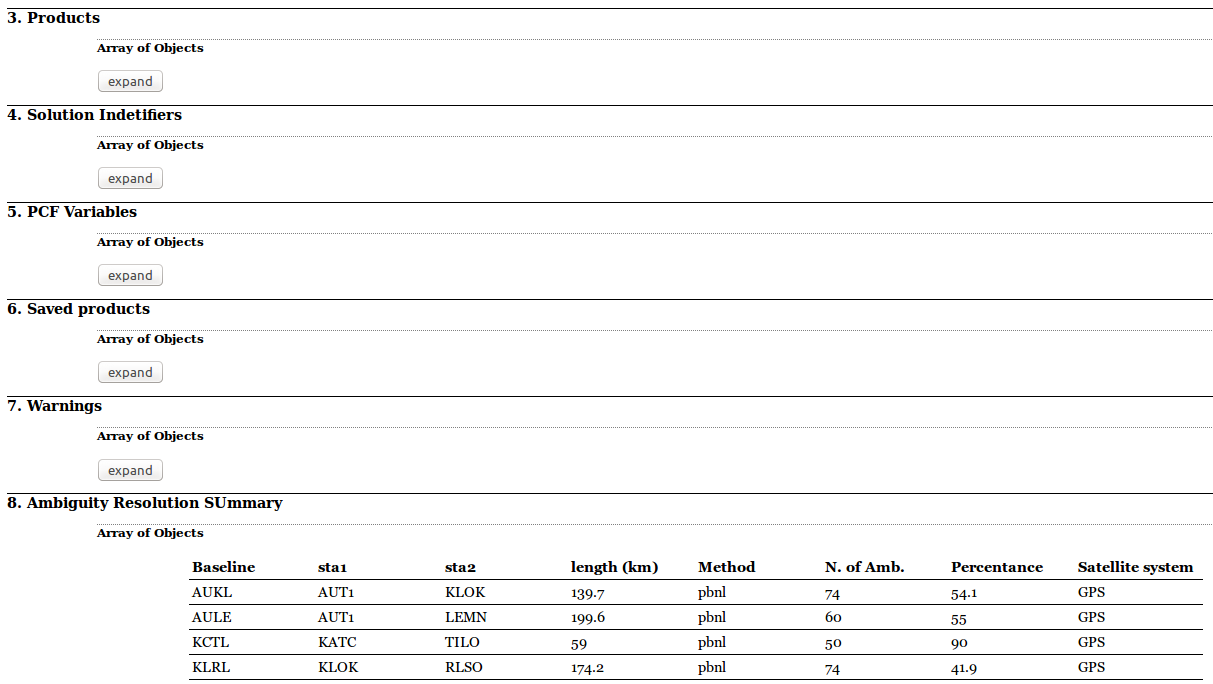
\includegraphics[height=.9\paperheight,width=.9\paperwidth]{jsonprint.png}}
\vskip-1.5cm
\begin{frame}\frametitle{Results \& Output}\framesubtitle{}
\begin{center}
\vskip -1.6cm
\begin{tikzpicture}
  \node (img1) {\shadowbox{\color{black!35}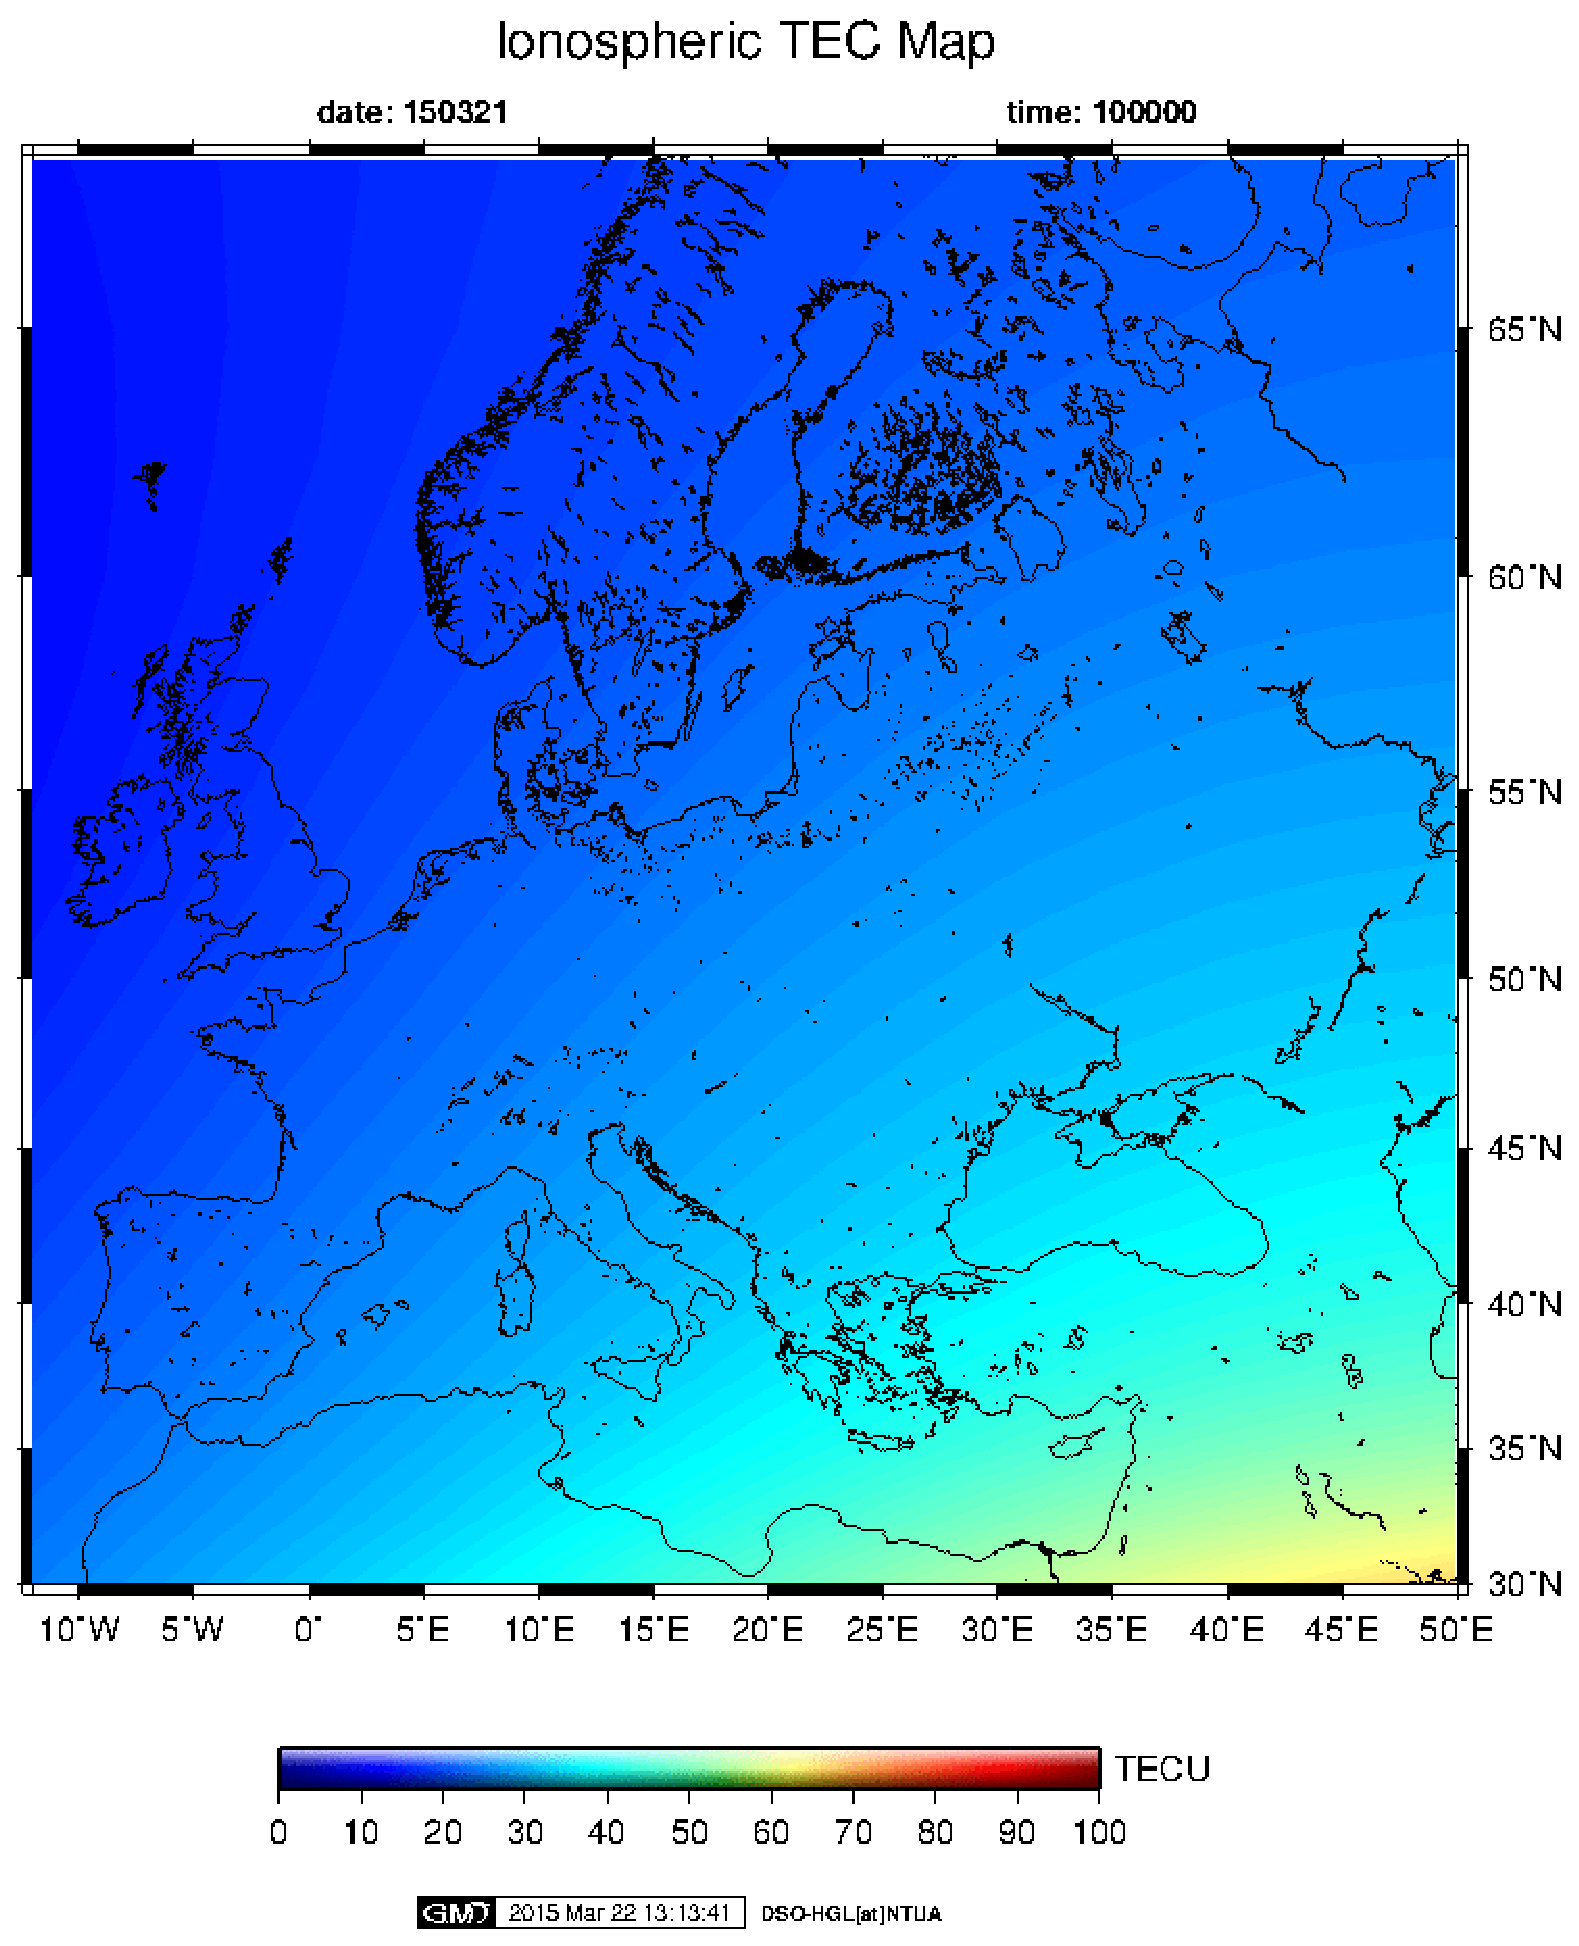
\includegraphics[height=4cm]{iono.eps}}};
%   \pause
  \node (img2) at (img1.north east) [yshift=-1cm,xshift=2.7cm] {\shadowbox{\color{black!35}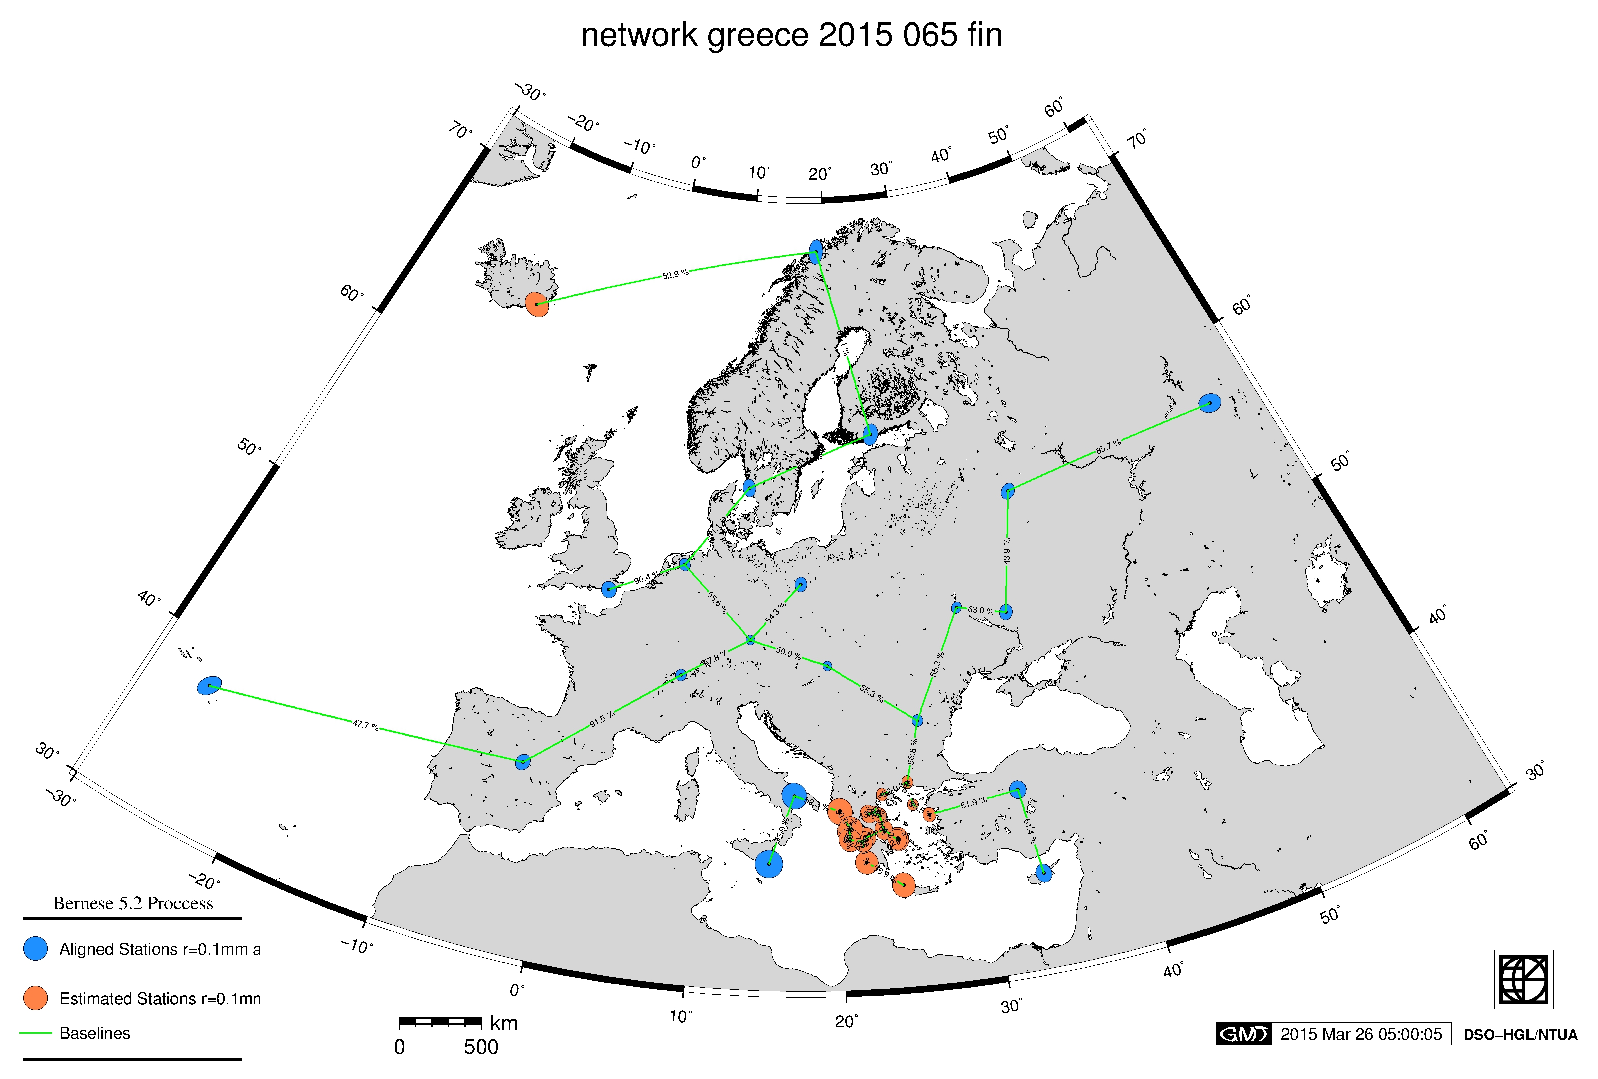
\includegraphics[height=2cm]{baseline.eps}}};
%   \pause
  \node (img3) at (img2.south) [yshift=-1.5cm,xshift=-.5cm] {\shadowbox{\color{black!35}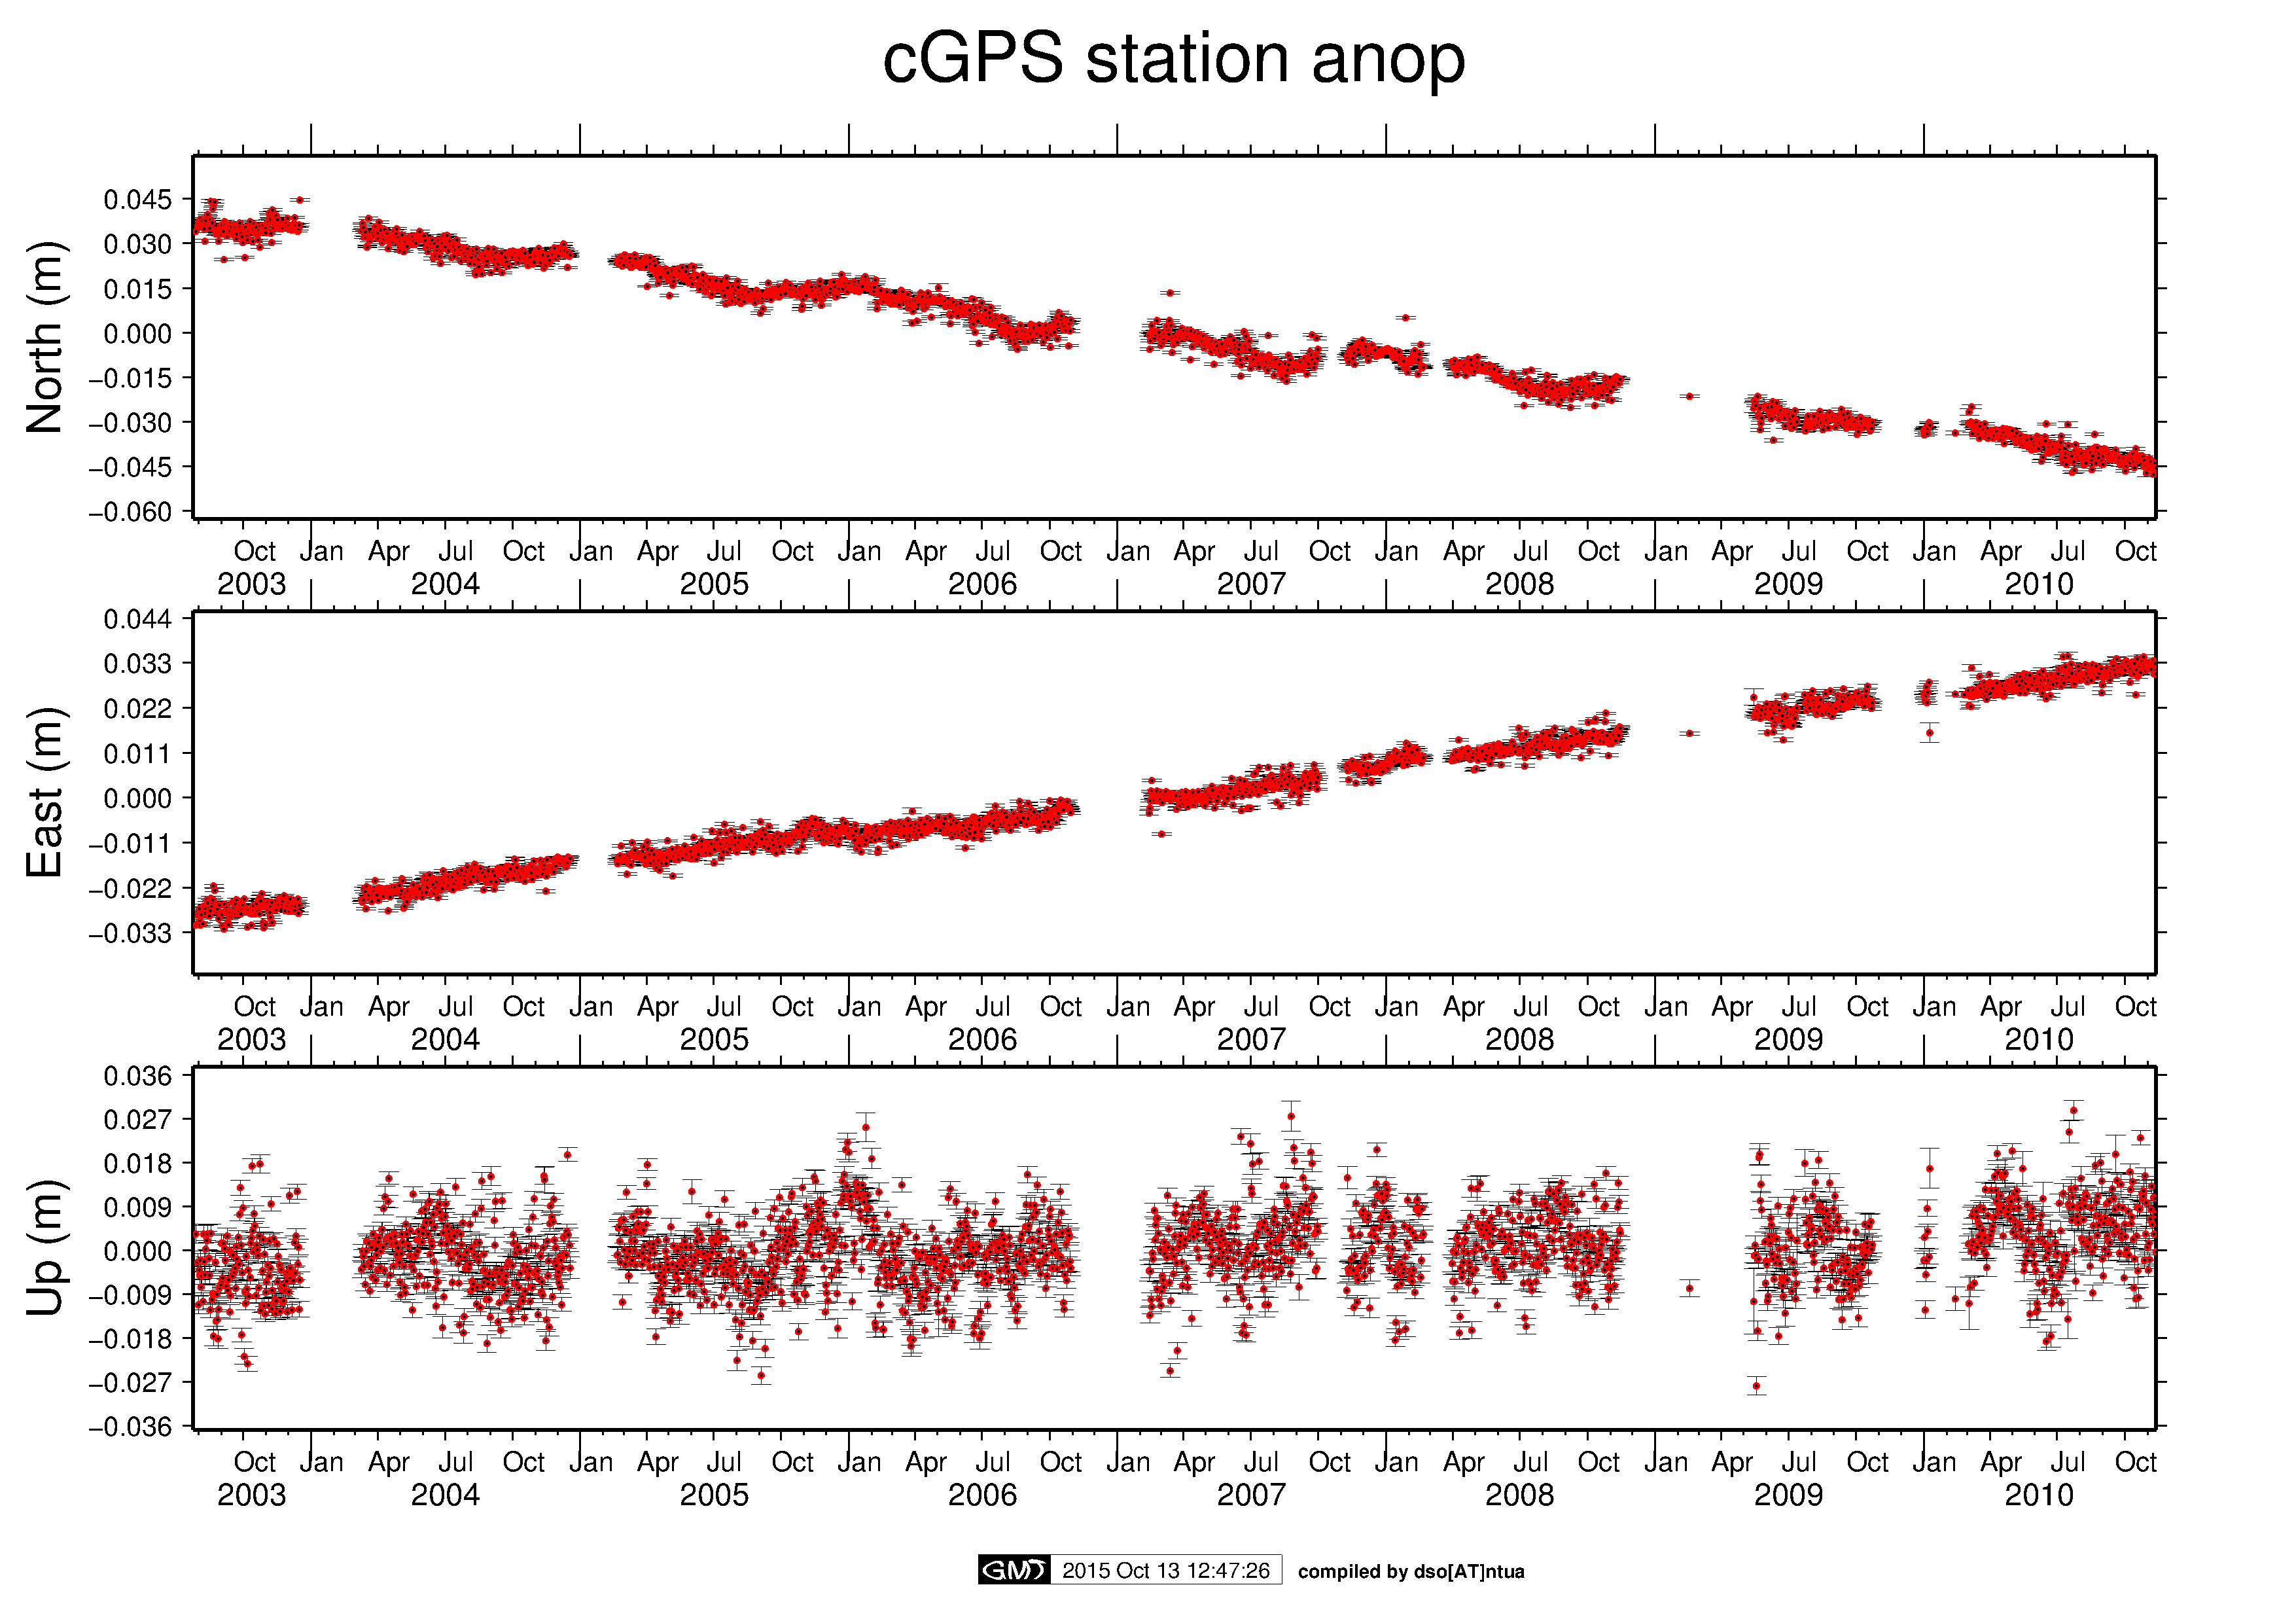
\includegraphics[height=2.6cm]{anop-raw.png}}};
%   \pause
%   \node (img4) at (img2.south west) [yshift=2cm] {\includegraphics[height=4cm]{img/dsoprint.png}};
\end{tikzpicture}
\end{center}
\end{frame}
}

% ------------------------------------------------------------------------------
\begin{frame}
  \frametitle{Coordinate estimates - Time series analysis}
  \framesubtitle{}
  \label{}
  \vskip-1cm
  \begin{columns}[T]
    \begin{column}{.4\textwidth}
      \footnotesize{
      We analyze time-series using in-house software tools, to estimate:
      \begin{itemize}
        \item tectonic velocities (linear trends),
        \item offsets/jumps due to miscellaneous reasons (e.g. instrumentation 
          changes, earthquakes, etc); note that this step requires a-priori 
          knowledge of such events (log-files, NOA earthquake catalogue)
        \item harmonics signals (using periodograms),
        \item velocity changes (e.g. inflation of Santorini isl.),
        \item post-seismic decay (still under development)
      \end{itemize}}
    \end{column}
    \begin{column}{.6\textwidth}
      \begin{center}
        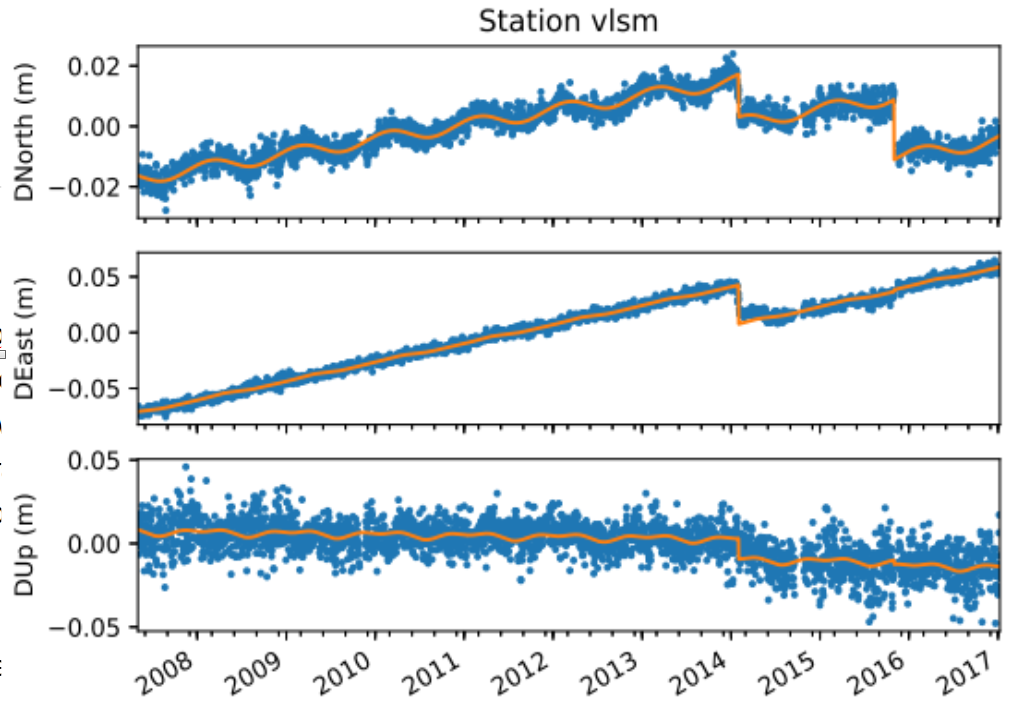
\includegraphics[width=\textwidth]{vlsm_ts.png}
      \end{center}
    \end{column}
  \end{columns}
 
\end{frame}
\note{}

 % ------------------------------------------------------------------------------
\begin{frame}
  \frametitle{Velocity field in Europe - Densfication project}
  \framesubtitle{}
  \label{}
  \begin{center}
    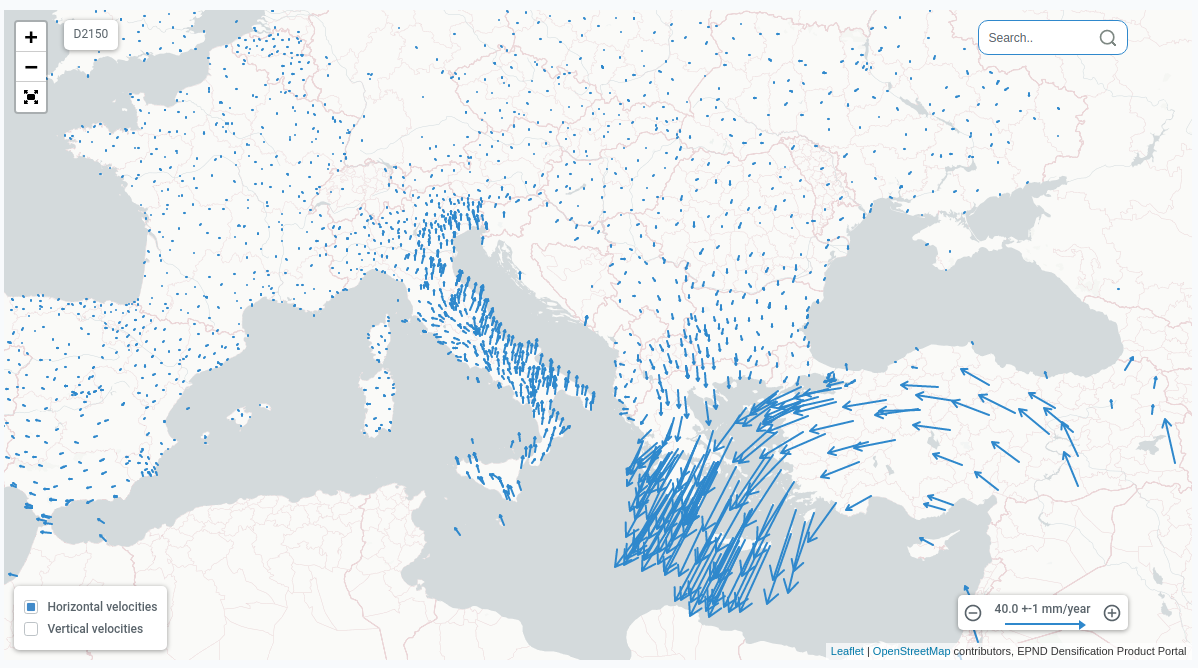
\includegraphics[width=.75\textwidth]{epndens_vel.png}
    \url{https://epnd.sgo-penc.hu/velocities/}
  \end{center}
\end{frame}
\note{}


 % ------------------------------------------------------------------------------
\begin{frame}
  \frametitle{Velocity field in Greece wrt a stable Europe}
  \framesubtitle{}
  \label{}
  \vskip-1cm
\begin{columns}[T]
  \begin{column}{.3\textwidth}
    \begin{center}
      \begin{itemize}\setlength\itemsep{1em}
        \item \~ 100 station
        \item data availability > 3 years
        \item Velocity field w.r.t. a stable Europe \citep{kreemer14}
      \end{itemize}
      \vskip1cm
      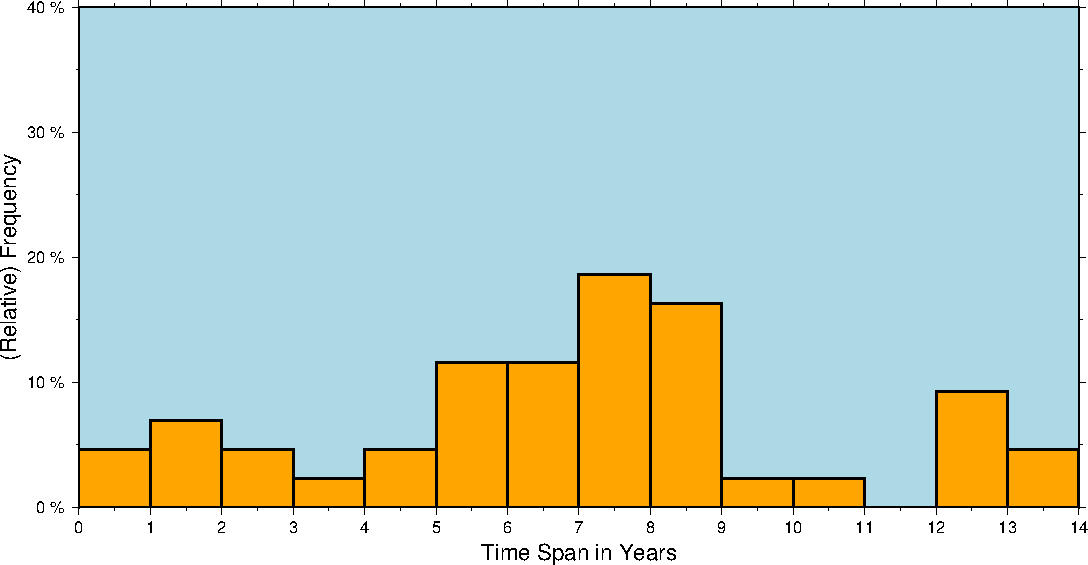
\includegraphics[width=.95\textwidth]{greece-freqs.png}
    \end{center}
  \end{column}
  \begin{column}{.7\textwidth}
    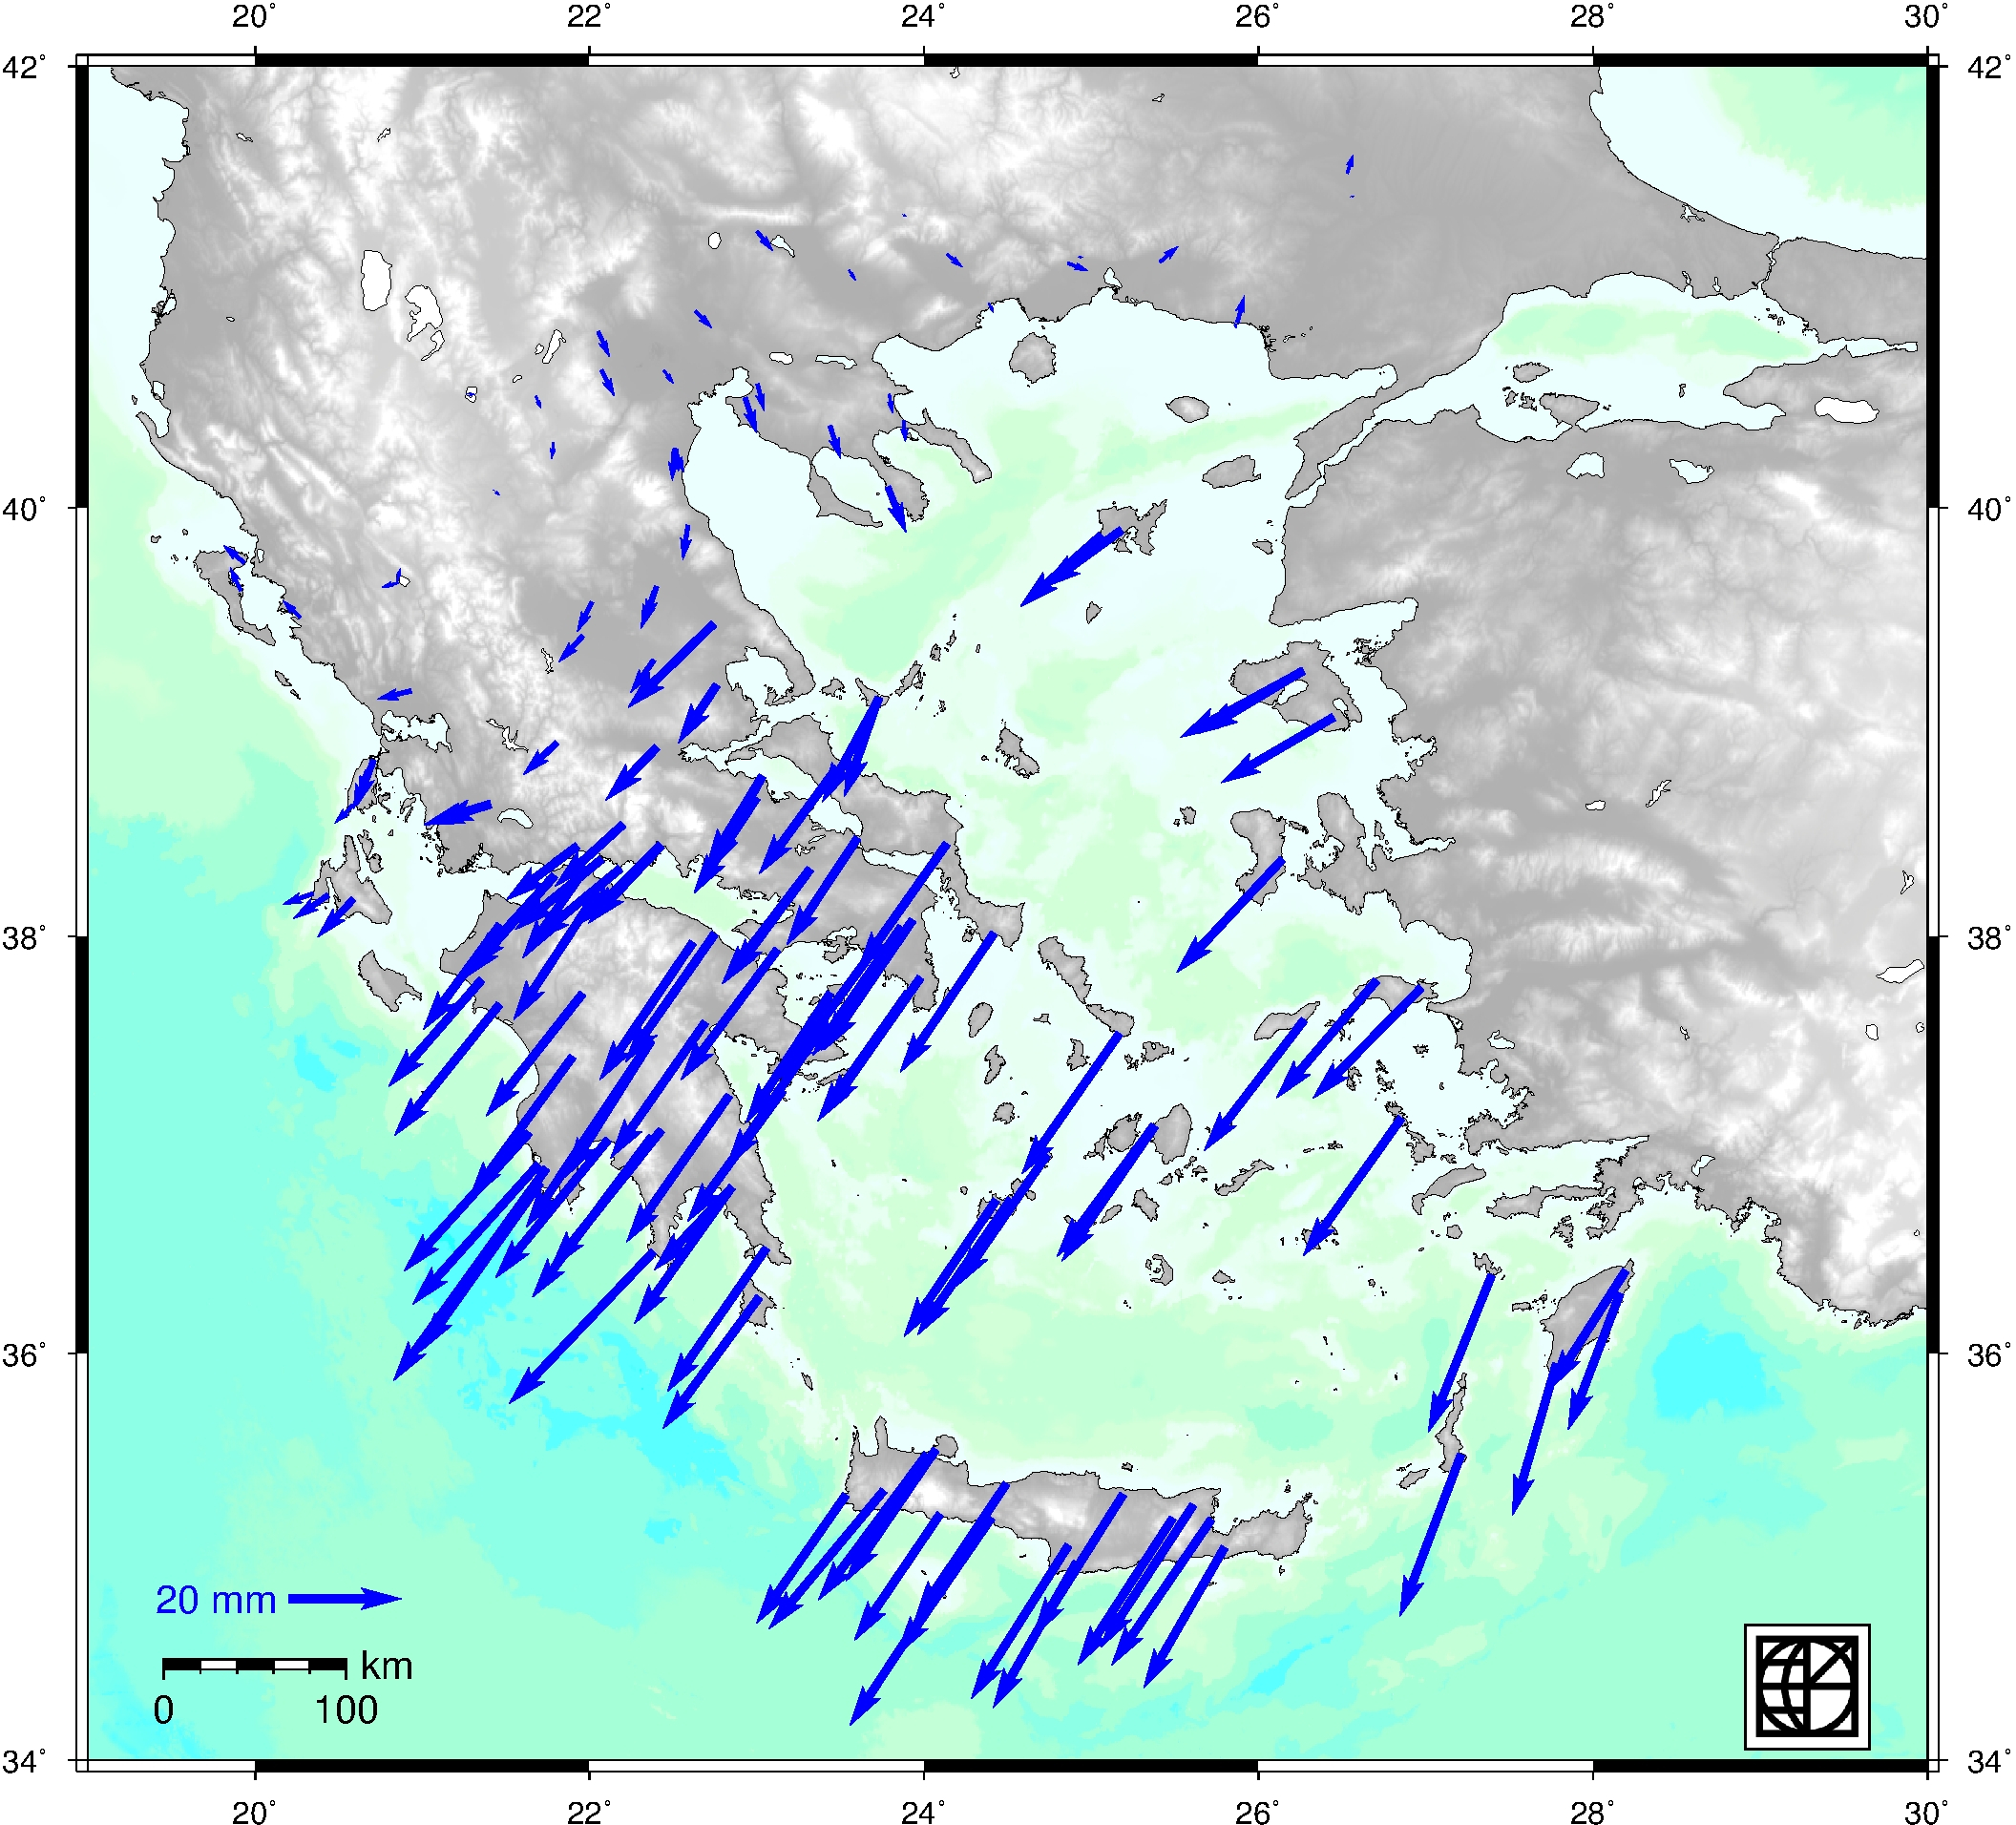
\includegraphics[width=.95\textwidth]{testvel.jpg}
  \end{column}
\end{columns}
\end{frame}
\note{}

 % ------------------------------------------------------------------------------
\begin{frame}
  \frametitle{Focus on specific regions - Corinth Gulf}
  \framesubtitle{}
  \label{}
  
  \begin{center}
    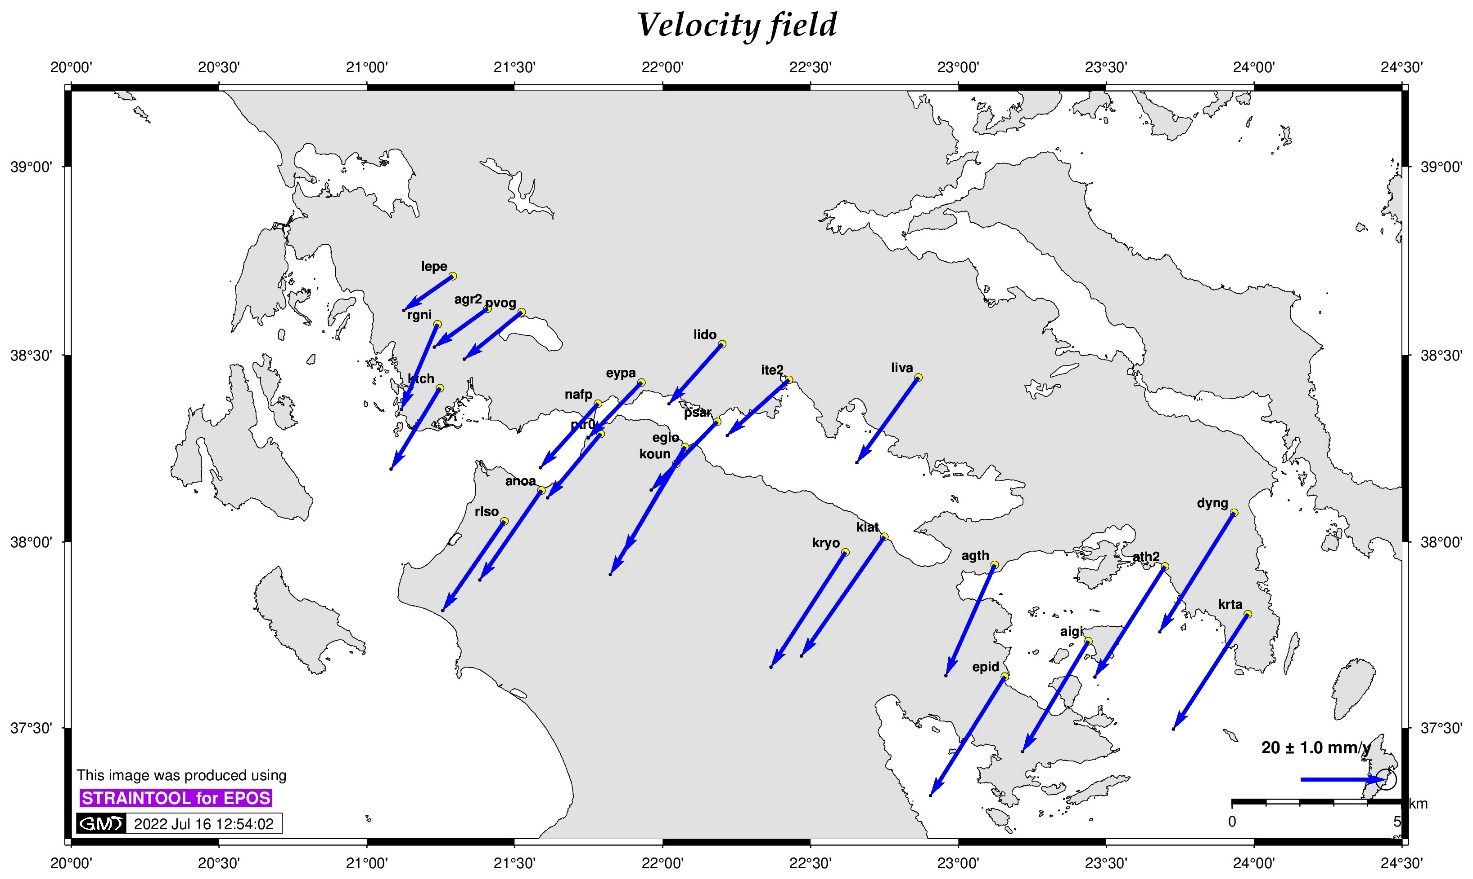
\includegraphics[width=.7\textwidth]{gsg2022_vel.jpg}  
  \end{center}

\end{frame}
\note{}

 % ------------------------------------------------------------------------------
\begin{frame}
  \frametitle{Recent Earthquakes}
  \framesubtitle{}
  \label{}
  \vskip-1cm
  \begin{columns}[T]
    \begin{column}{.5\textwidth}
    \begin{center}
 	  \textbf{Thessaly 2021} 
 	  
 	  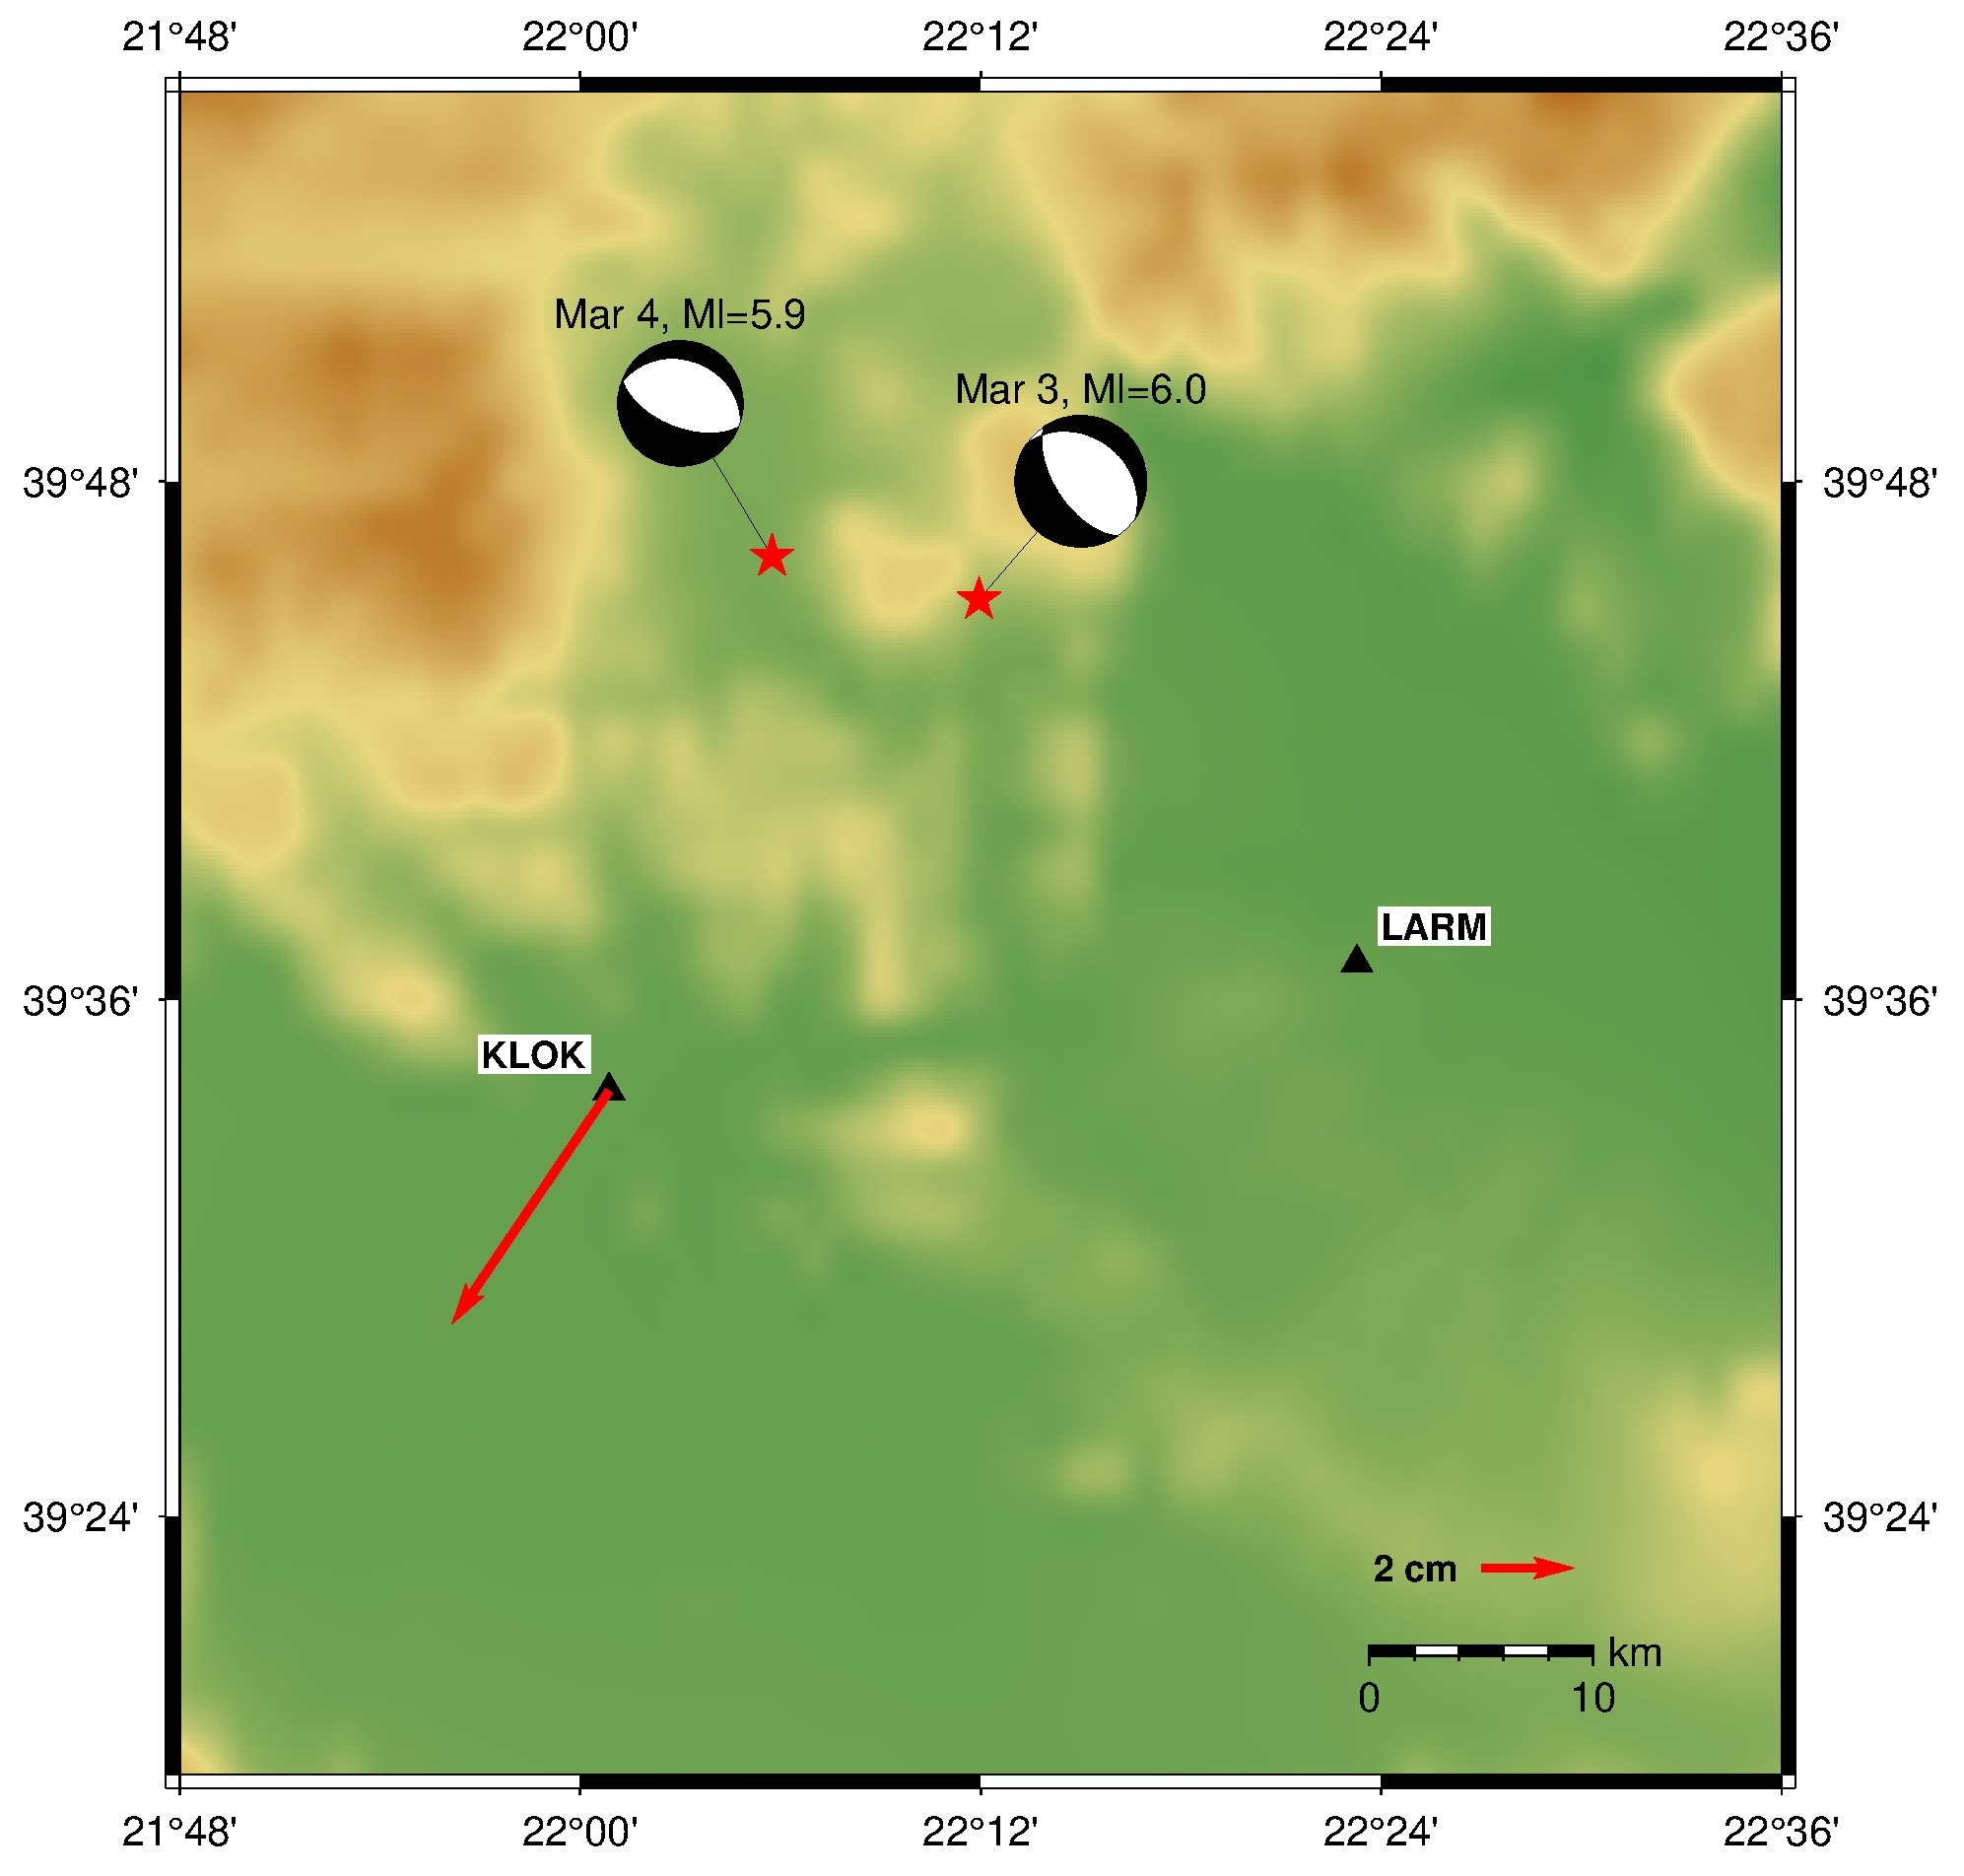
\includegraphics[width=.7\textwidth]{eq_elassona.jpg}    

      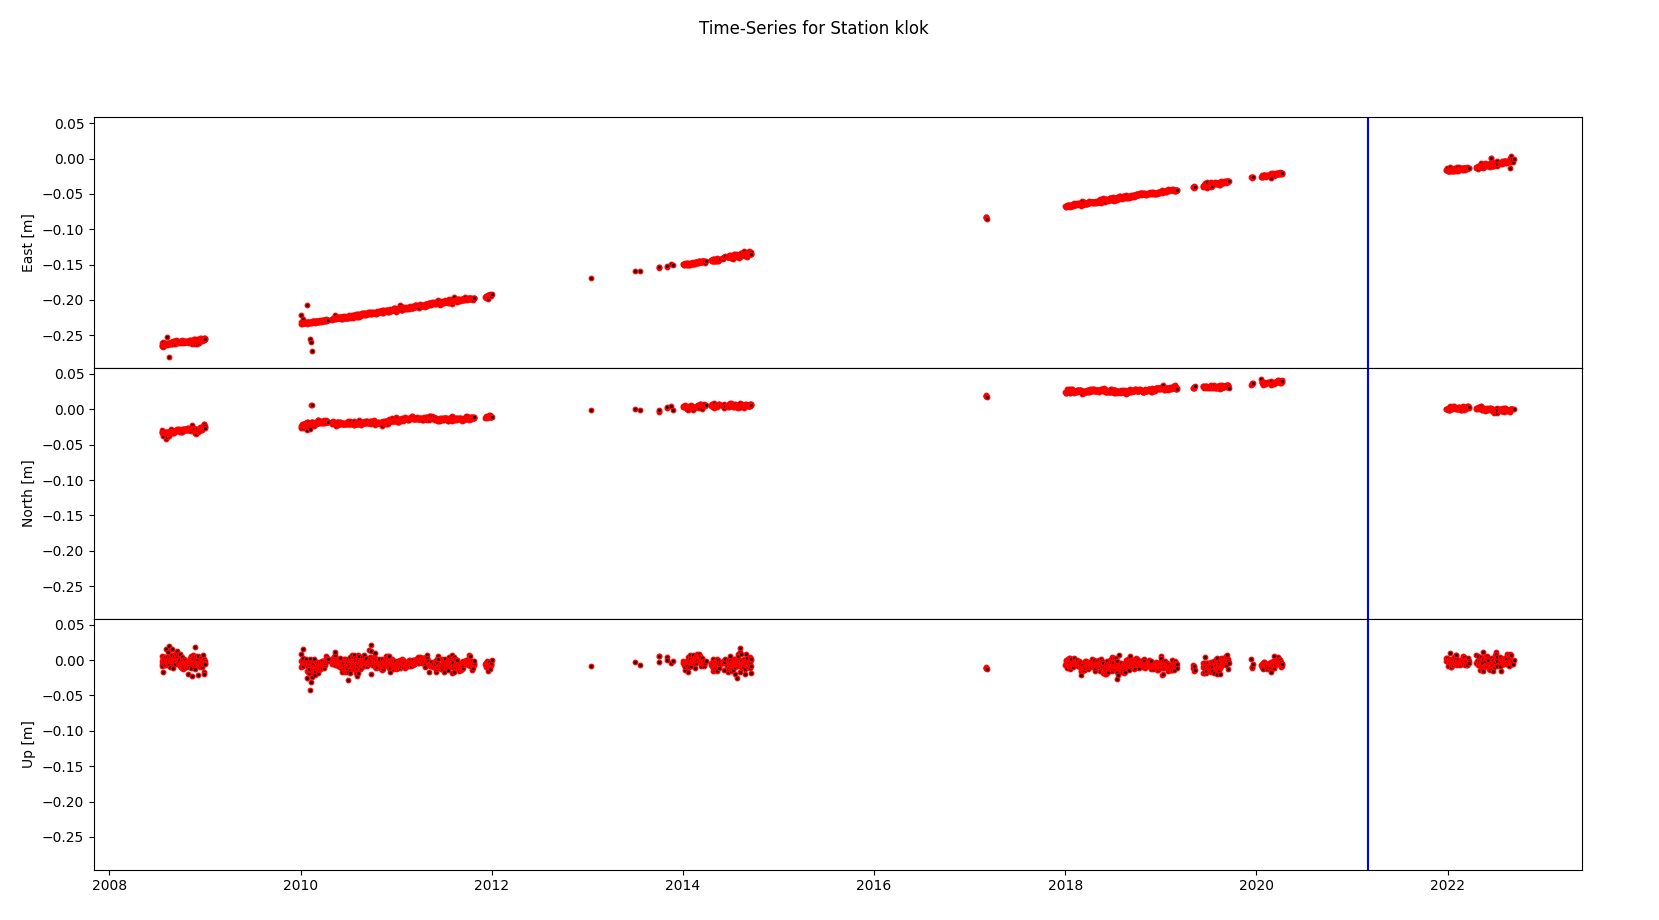
\includegraphics[width=.9\textwidth]{klok_ts.png}

    \end{center}

    \end{column}
    \textcolor{blue!40}{\vrule width 1pt}
    \begin{column}{.5\textwidth}
      \begin{center}
        \textbf{Itea 2022}
        
        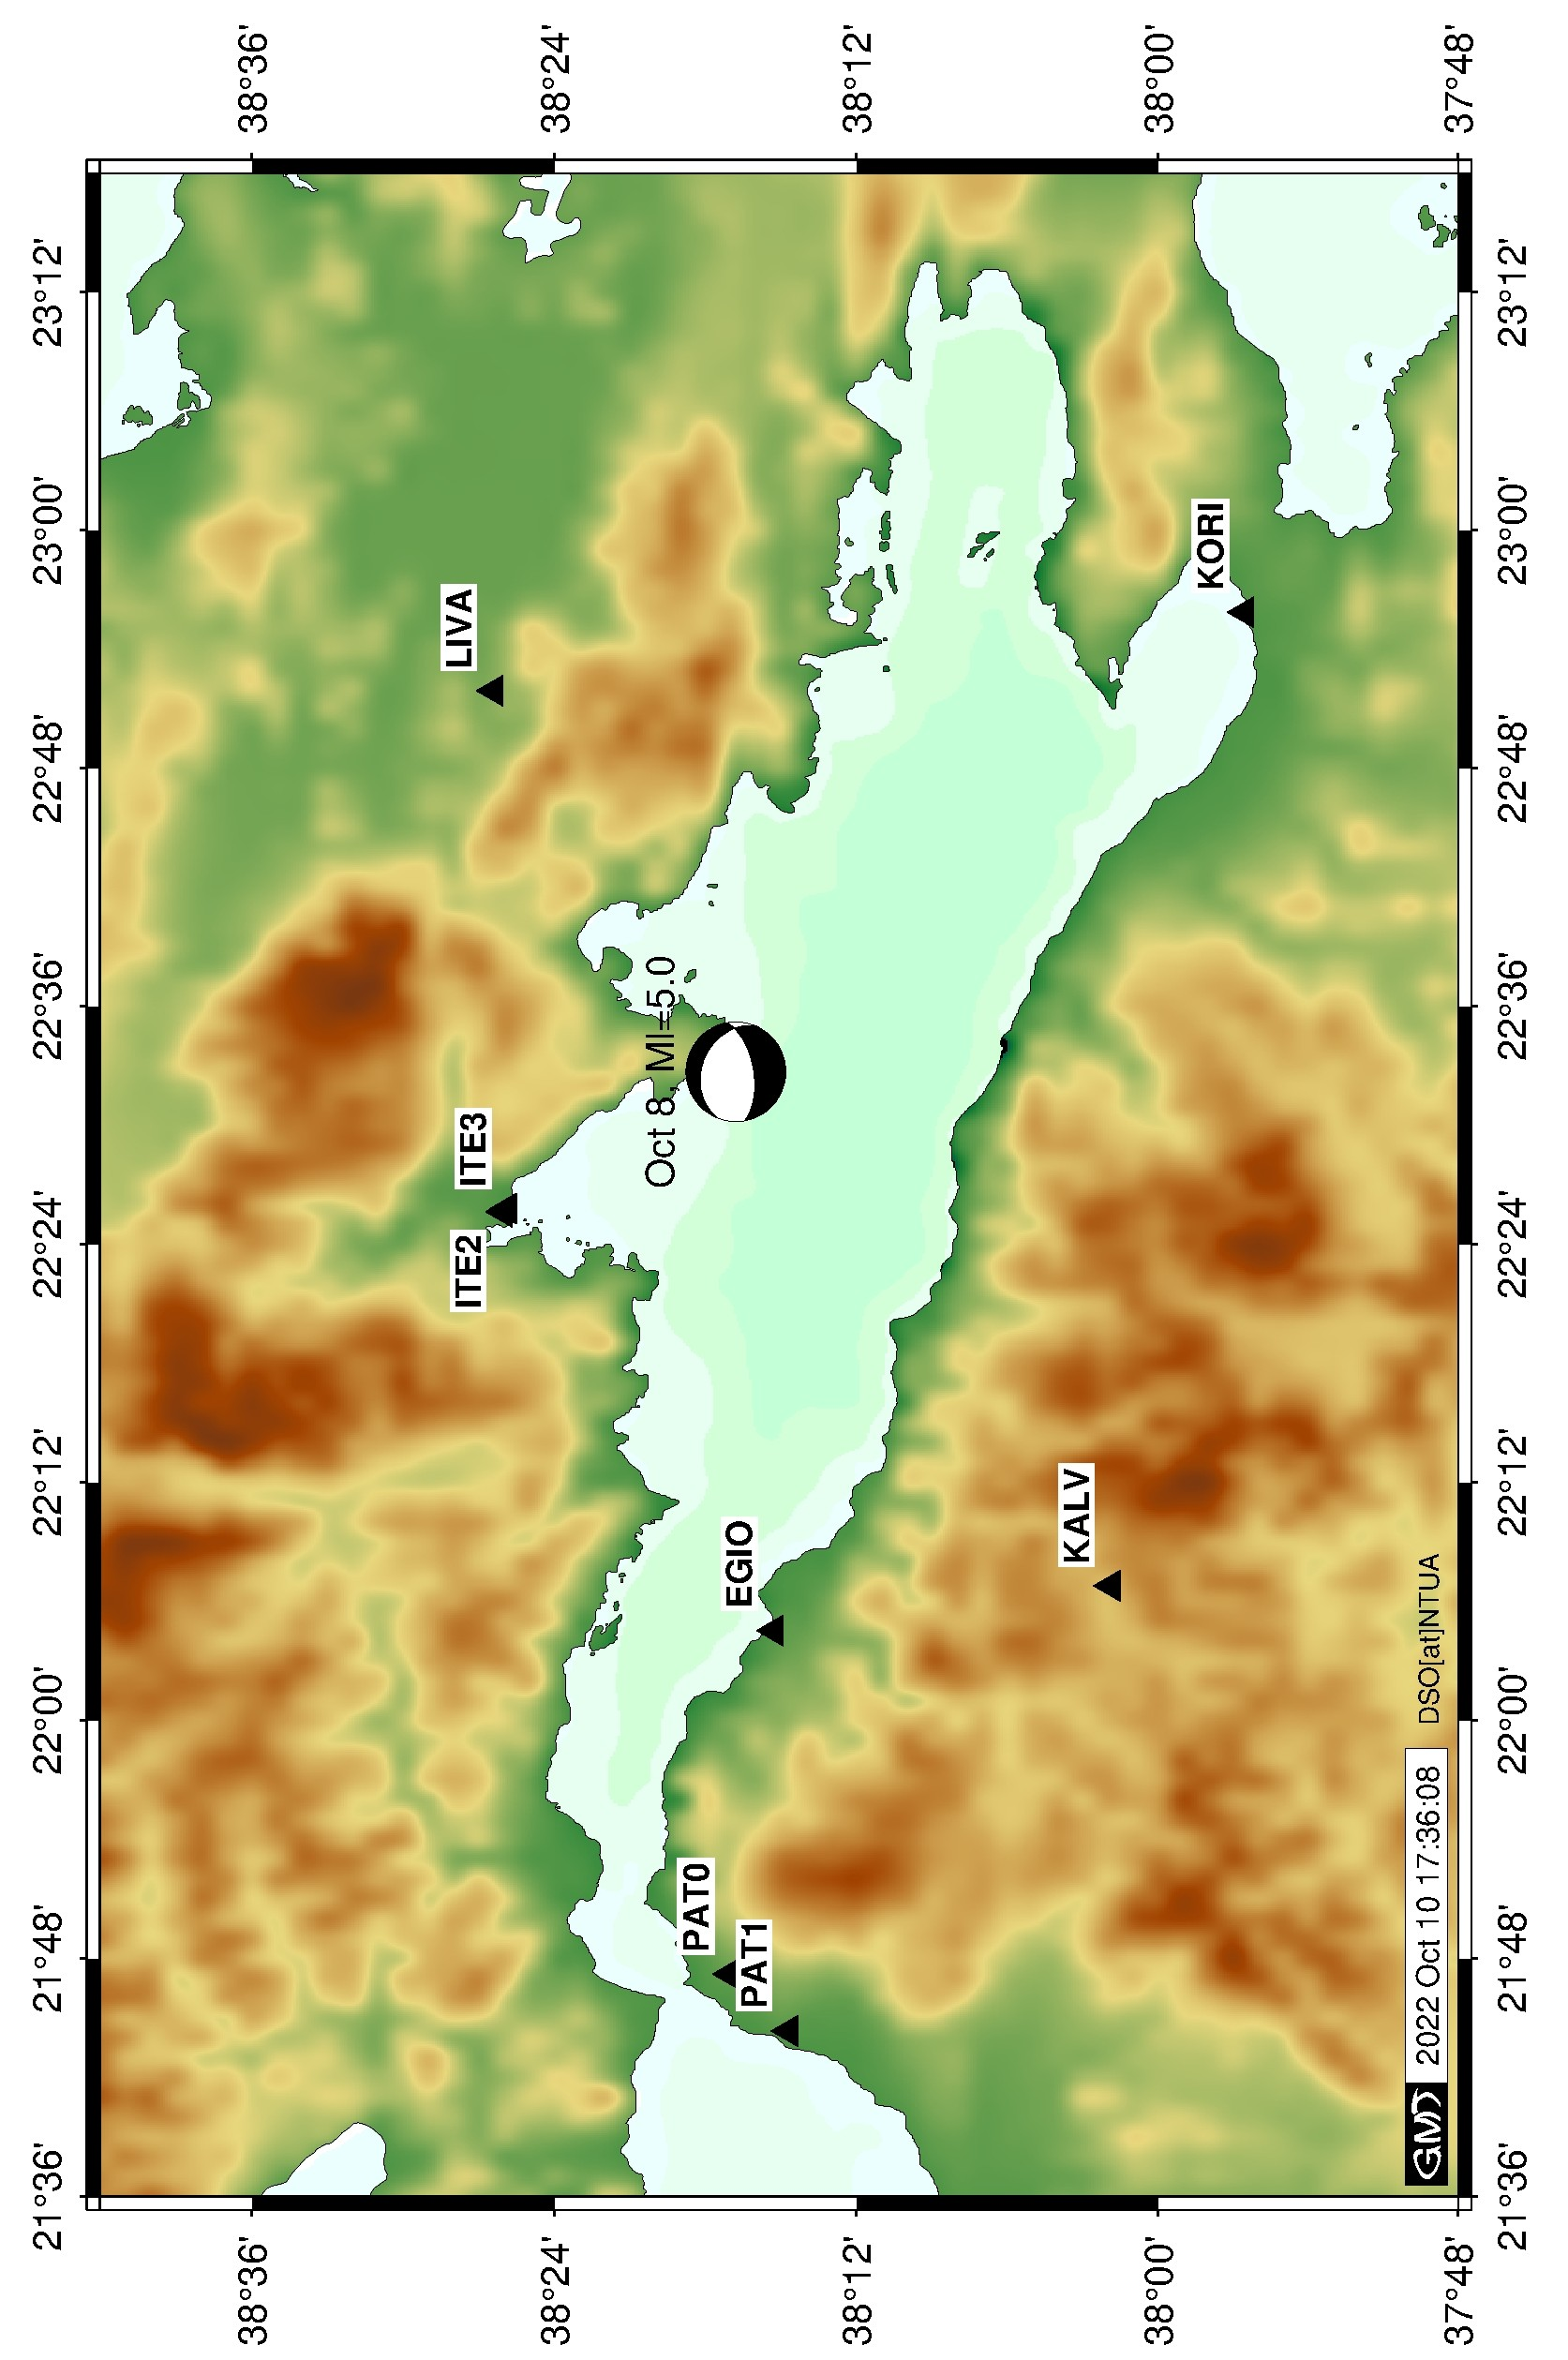
\includegraphics[angle=-90,origin=c,width=.9\textwidth]{eq_itea221008.jpg}
        \vskip-.5cm
        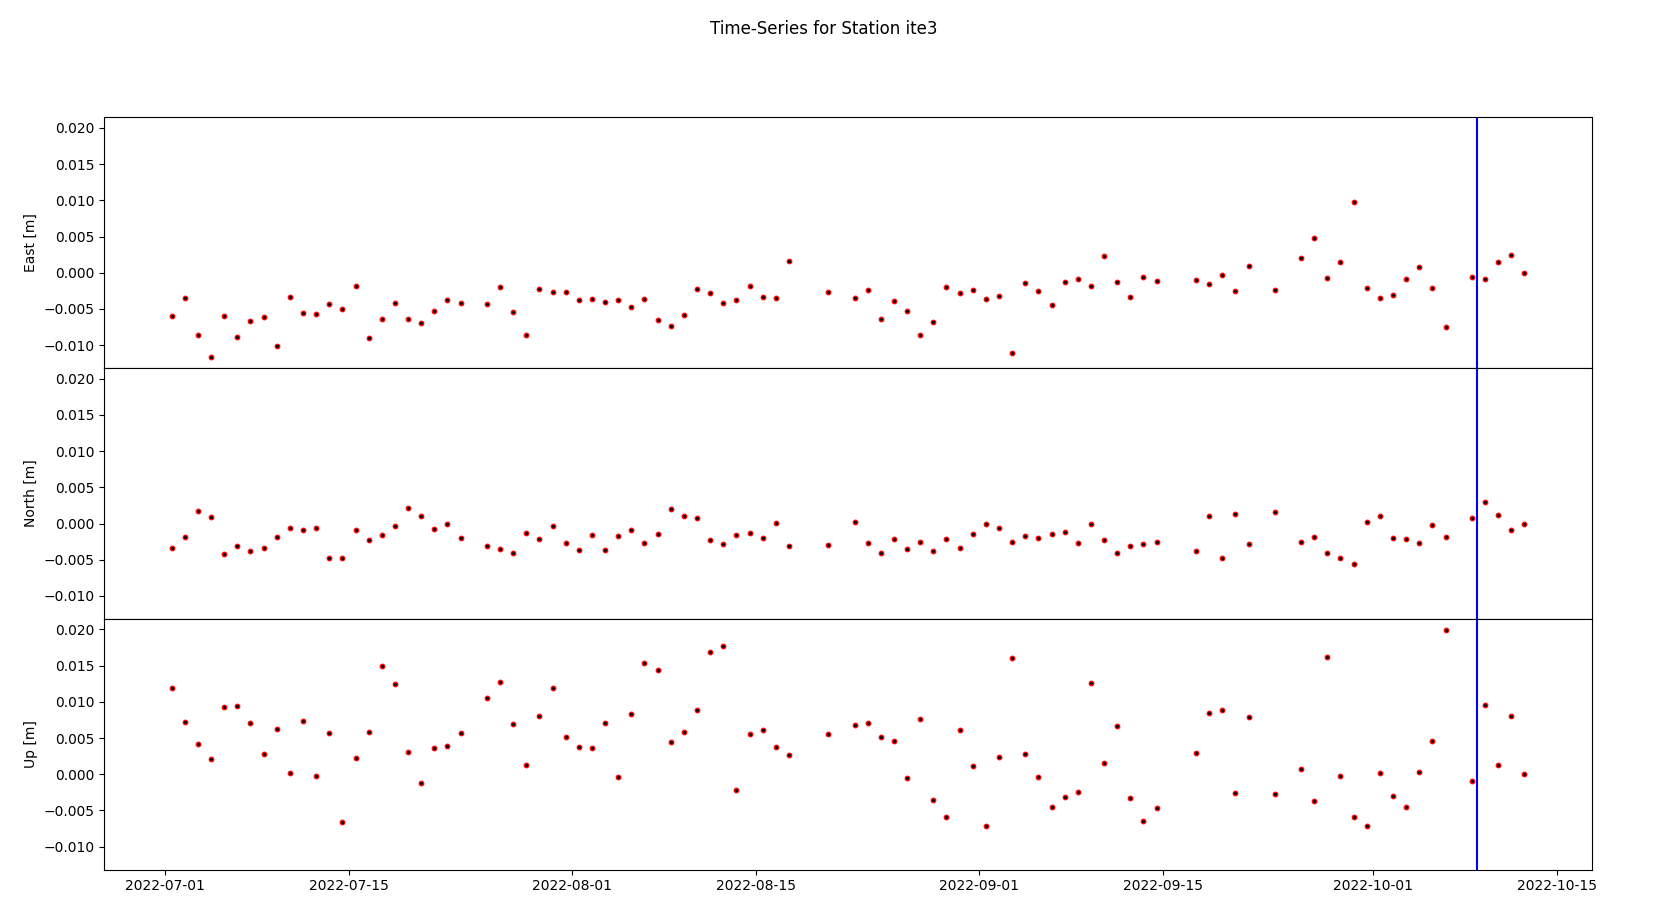
\includegraphics[width=.9\textwidth]{ite3_ts.png}
      \end{center}
    \end{column}
  \end{columns}
\end{frame}
\note{}

 % ------------------------------------------------------------------------------
\begin{frame}
  \frametitle{Strain rates}
  \framesubtitle{}
  \label{}
  \vskip-1cm
\begin{columns}[T]
  \begin{column}{.3\textwidth}
    \begin{itemize}\setlength\itemsep{1em}
      \item \textbf{StrainTool} software used to estimate strain tensor parameters \citep{straintool}
      \item grid step 0.5$^{\circ}$
    \end{itemize}
  \end{column}
  \begin{column}{.7\textwidth}
      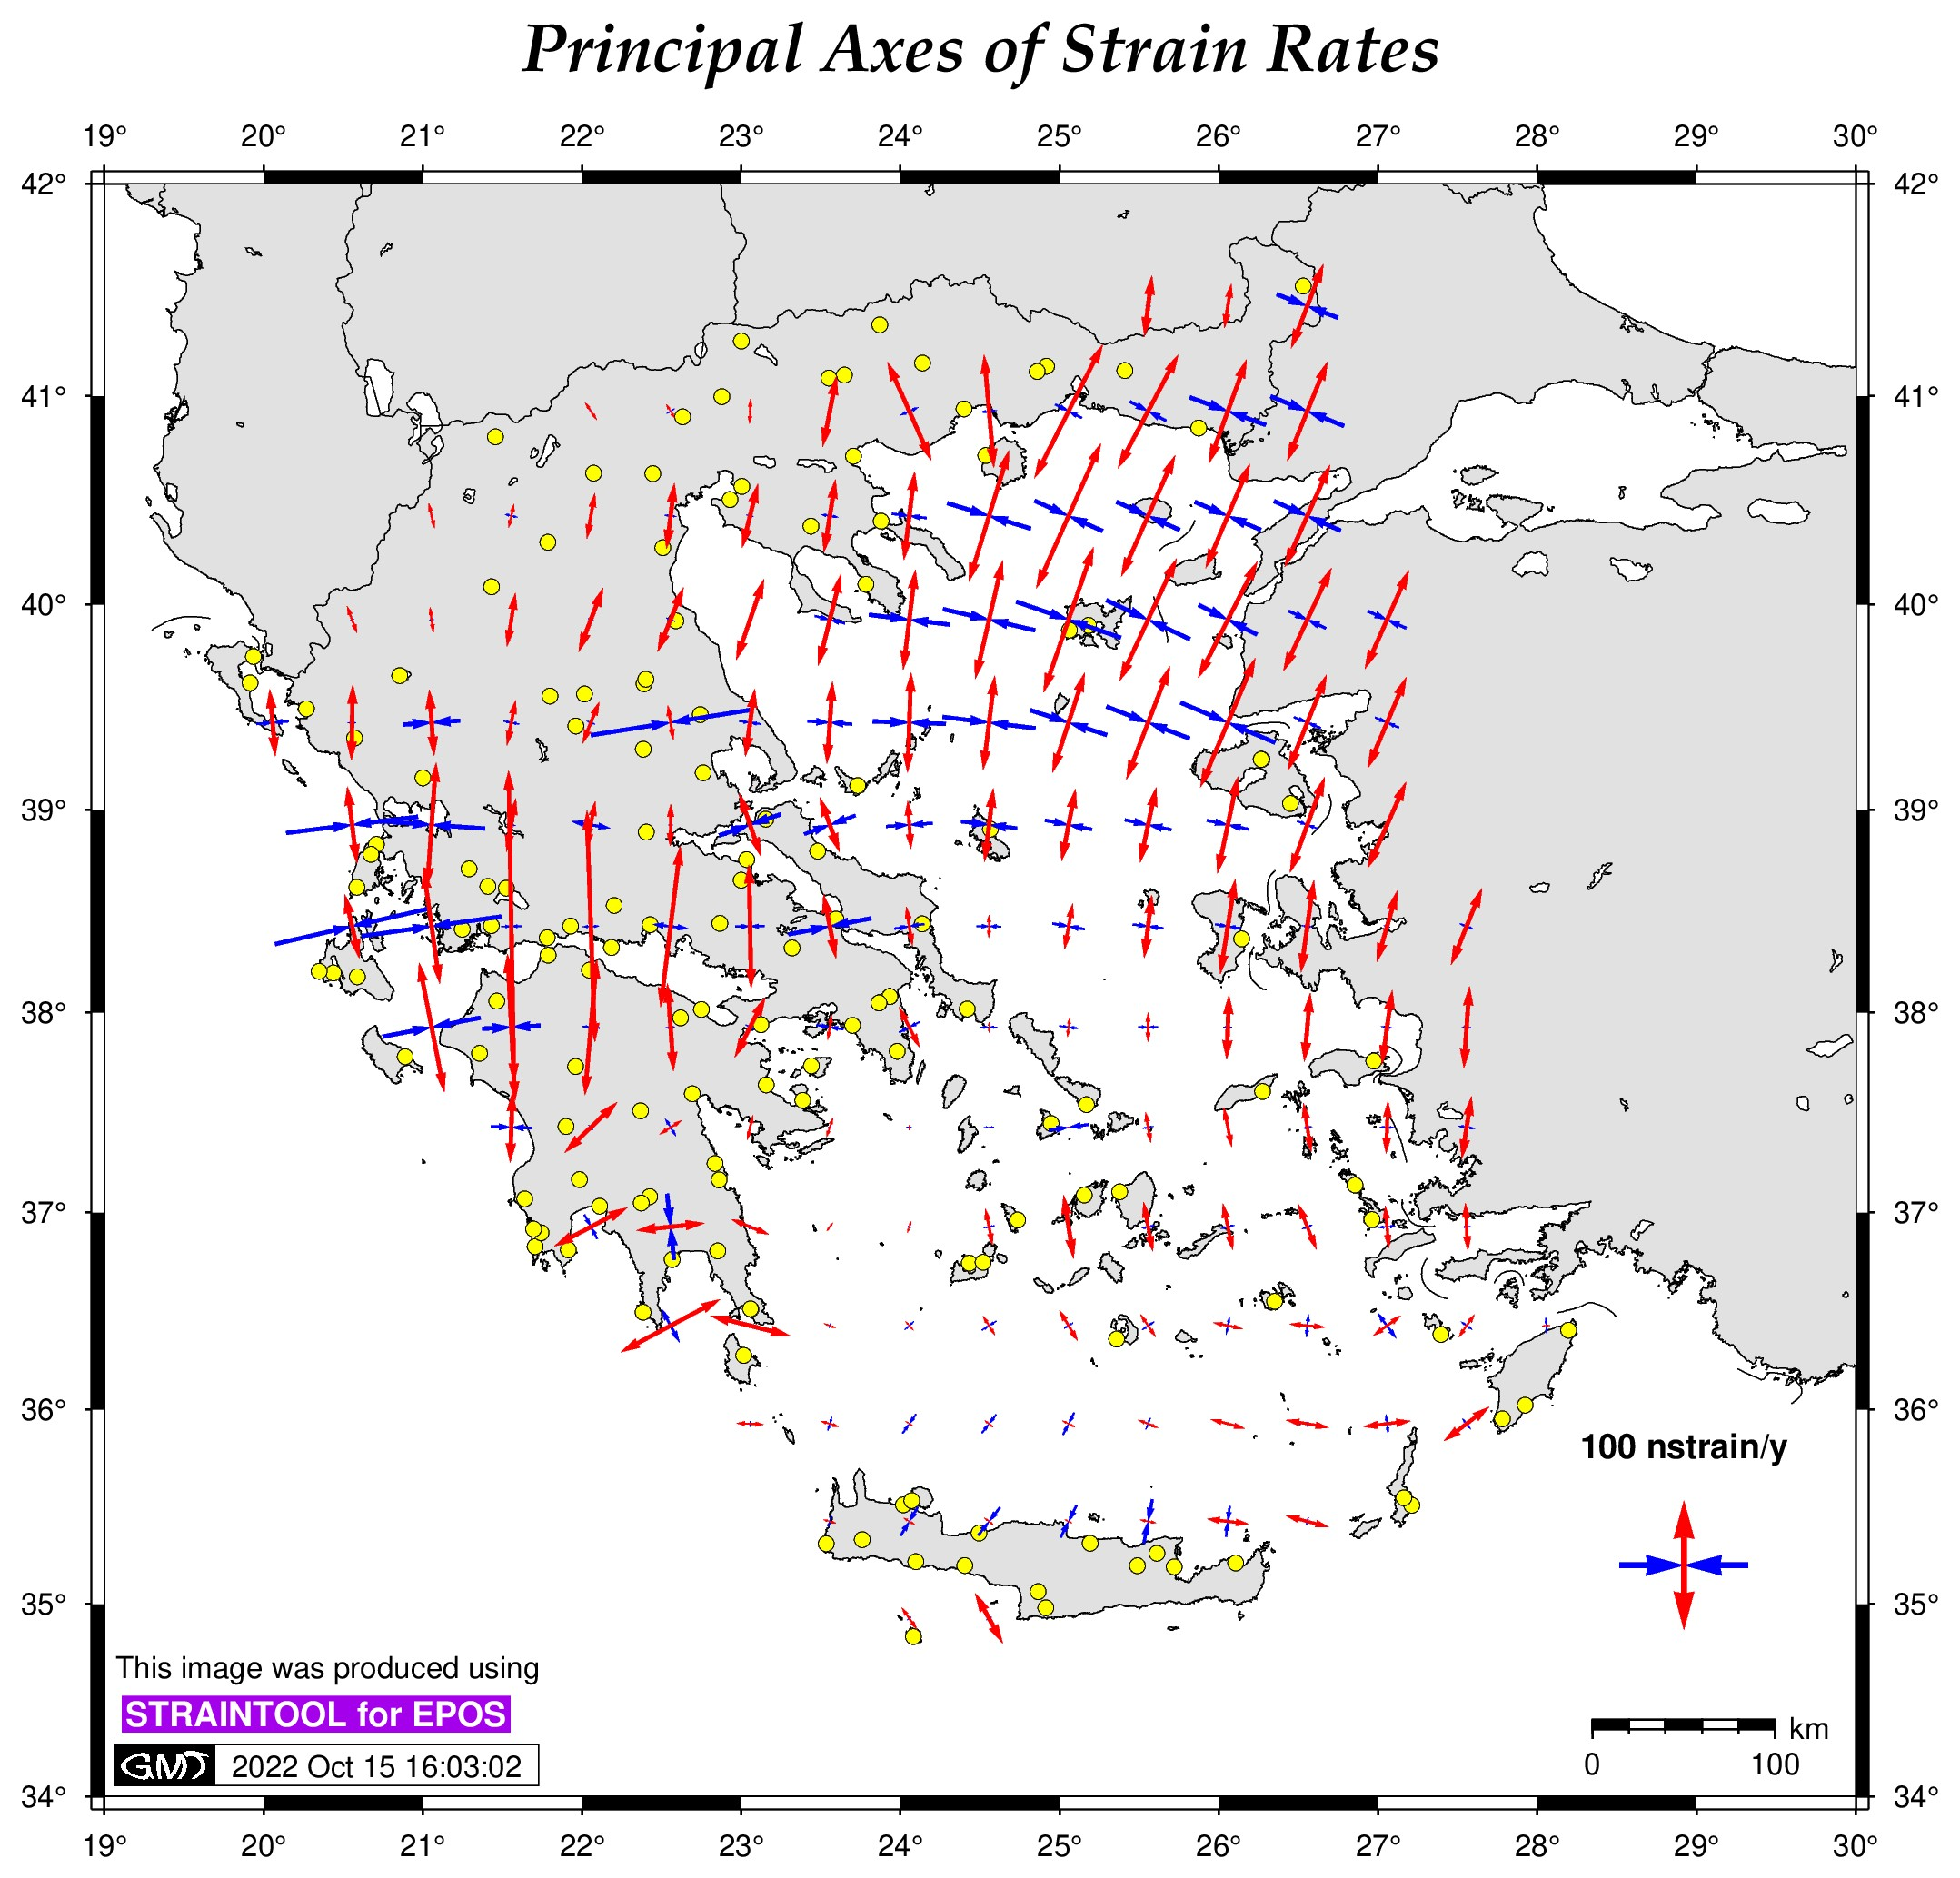
\includegraphics[width=.95\textwidth]{gr-output_str.jpg}
  \end{column}
\end{columns}
\end{frame}
\note{}

 % ------------------------------------------------------------------------------
\begin{frame}
  \frametitle{Strain rates - focus on specific region}
  \framesubtitle{}
  \label{}
  \vskip-1cm
\begin{itemize}\setlength\itemsep{.2em}
  \item 25 Permanent GNSS Station
  \item grd step 0.25$^{\circ}$
\end{itemize}
\begin{center}
  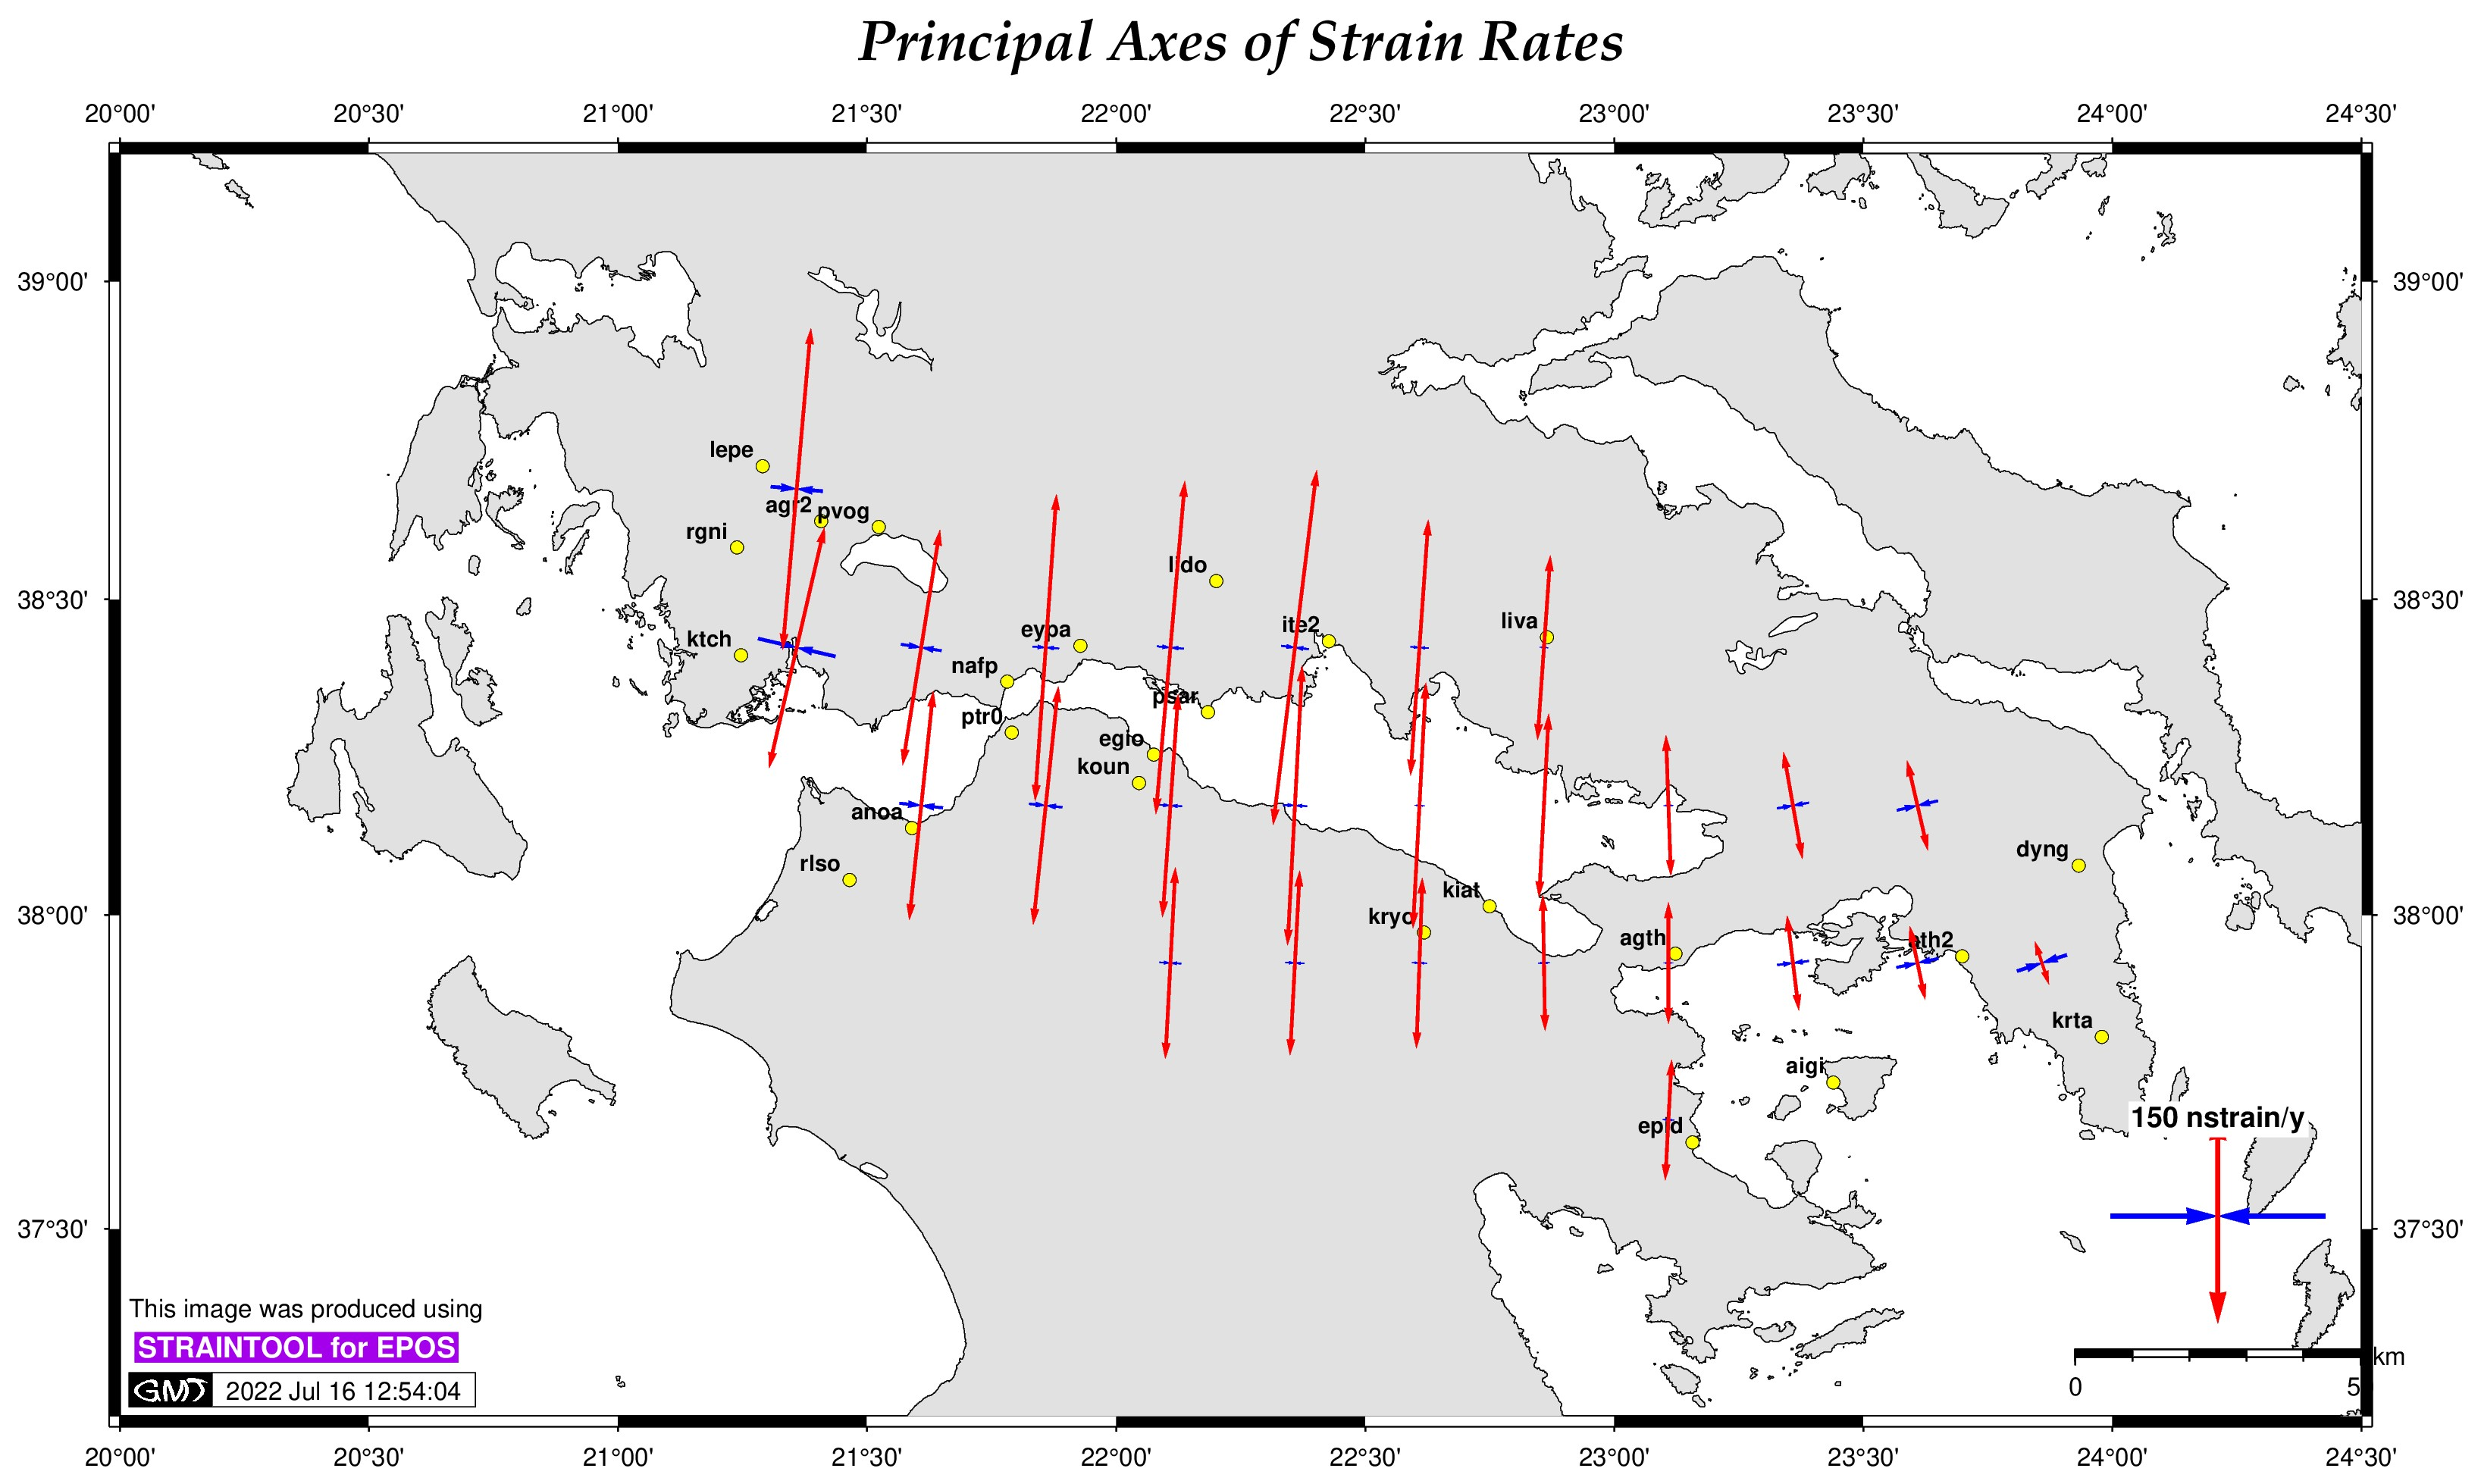
\includegraphics[width=.65\textwidth]{crfeu-output_str.jpg}
\end{center}

\end{frame}
\note{}





\section{Discussion / Conclusions}
 % ------------------------------------------------------------------------------
\begin{frame}
  \frametitle{Discussion / Conclusions}
  \framesubtitle{}
  \label{}
  \vskip-.5cm
  \begin{itemize}\setlength\itemsep{.5em}
    \item Greece is located in a complex tectonic background with many changes in the kinematics of the area.
    
    \item Routine processing and monitoring are very important and revealing for 
      Greece; products are requested by and disseminated to a wide range of Geoscientists.

    \item Greece's crustal dynamics are evidently complex and inhomogenous; a difficult 
      task to model by Reference Systems (especially non-dynamic, such as the ones 
      currently in use).

    \item A dense velocity field for accurate estimation of ground/tectonic motions in the region will help to develop a stable local reference frame and the connection of the region with the global and European reference systems.
    
    \item The continuous monitoring of the networks gives useful results for the effect of strong earthquakes or other ``abrupt'' phenomena; small, dense networks 
      are of great help (even with instrumentation of non-geodetic accuracy).
  \end{itemize}
\end{frame}
\note{}

